\newacronym[plural=APIs,firstplural=Application Programming Interfaces (APIs)]{api}{API}{Application Programming Interface}

% \newacronym{svg}{SVG}{Scaleable Vector Graphics}

% \newacronym{kvm}{KVM}{Kernel Virtual Machine}

% \newacronym{wsgi}{WSGI}{Web Server Gateway Interface}

\newglossaryentry{pubsub}
{
    name=Pub/Sub,
    description={Publish/Subscribe messaging system in which publishers blindly send their message to a certain topic while subscribers can express interest in one or more topics to get the messages send by the publishers.}
}

\newglossaryentry{os_ring}
{
    name=protection ring,
    description={Mechanism to protect software systems by decreasing permissions to access functionality with each ring layer, starting at ring 0 (all permissions).}
}

% \newacronym[longplural={Frames per Second}]{fpsLabel}{FPS}{Frame per Second}

\begin{thesis}{Adrien: Gamification of Interfaces for Learning and Performance Enhancement}{Adrien LEFEVRE}{chapters/00_abstract_resume}{adrien.jpeg}{}
    \chapter{Introduction}

\section{Context}

The learning-performance distinction is a concept in behaviorism that stresses the difference between the learning of a behavior and actual performance of the behavior. Learning is a change in the ability and potential to do when the performance consists of an execution of the learned behavior. \cite{kantak2012learning}

This distinction is significant in subjects involving physical movements attached to something else, an idea, image, or sound, for example, in music or language learning.

The relative persistence of learning is sometimes referred to as an enhanced capacity for motor skill performance. \cite{kantak2012learning}

These subjects are traditionally challenging to learn because integration with performance takes much time. Acquiring expertise in the practice of a discipline through repetition can be laborious. People get bored.
With training, the learner can perfect their ability to link an idea, a wished sign, a sound, a mental image with a movement, or a "physical" sound. Performance psychology is the scientific field describing the human ability to translate mental concepts into physical or musical practice.

\section{Field of research}

The domain of gamification looks at how to make people less bored when learning subjects by introducing playful mechanisms \cite[]{saleem2022gamification}.
In recent years gamification has revolutionized the field of professional training. It has accompanied the digital transformation of training and modernized existing modules. This principle of gamification has brought real advantages to learning mechanisms by combining pleasure and skill acquisition.

The gamification of training corresponds to a set of playful mechanisms designed to "gamify" learning content to personalize the relationship with training. This technique improves learner engagement by arousing their interest. Being immersed in an enjoyable educational experience enrich the memorization process thanks to the emotional trigger provided by the game. The playfulness of training will encourage positive emotions that lead to the improvement of learning. The effect is engagement and motivation improvement.

Another way to improve engagement is through activating different senses. In the HCI field, Augmented Reality and Tangible Interfaces make digital information more immersive by projecting it into the real world, engaging sight, sound, and kinesthesia \cite{seichter2007augmented}.

The Augmented Reality (AR) experience is thriving as a significant trend. Around 2.4 billion people use AR on their mobile worldwide in 2023. AR can augment computer-generated graphics into the natural environment on screen. This augmentation can serve gamification, improving the education system efficacity and making students' attitudes more positive. It makes learning interesting, fun, and effortless, improving collaboration and capabilities.

These paradigms make the link between abstract information and the body more legible.
HCI optimizes the symbiosis between user and technology (Human-Computer Confluence) or how the elements of the human ecosystem cooperate to optimize their interaction with humans. Communication Technology (ICT) can be based on radically new forms of sensing, perception, interaction, and understanding \cite{ferscha2007human}. The particularity of digital learning environments lies in the fact that they can accommodate diverse users' needs \cite{stephanidis2019seven}.

This thesis takes inspiration from work in gamification, performance psychology, and AR/Tangibles. This thesis reflects on how to learn by exploiting these different domains.

\section{Approach}

We have thus carried out several projects within the framework of studying a user's ability to learn and perform with the help of an augmented or tangible interface.

These projects aim to exploit specific human ways of interacting to promote using different intelligences, thus the retention of information and the ability to practice efficiently. 

The devices that users interact with use augmented reality, sound, visual feedback, haptics, and enhanced features through electronics or software to help motivate them.

\section{Contributions}

The areas studied are: learning the basics of music theory using an interactive electronic score, practicing music through augmented reality learning applications, and learning and practicing sign language through a video game and an AR training application.
    % \chapter{Robotics middleware}



\section{Introduction}

Robotic systems require complex infrastructure to be able to operate correctly. With numerous different parts working together that have to communicate and coordinate, these systems need a robust way to enable such communication. At the same time, translating user commands into instructions that can be understood by the inner electronics of the robot is a complex process that should only be exposed to qualified operators.

Robotics middleware is a type of software that provides utilities to software applications used in complex robot control systems. It is sometimes referred to as "software glue" because it links together different software components to create a complete system. Using a robotics middleware is a solution to the problems defined above: the middleware facilitates communication, provides a way to package software in a structured manner, and enables hardware abstractions to make development easier.

In this chapter, we introduce ALFRED as a robotics middleware. It follows the structure of UNIX-like operating systems, with separation of privileges between system programmers and normal users. It enables communication between software components with an external message passing system. It allows robotics application designers to create interactions with robotic arms without the need for specialized education or to learn the inner workings of a robotic arm. Finally, it provides access to software utilities and a hardware abstraction layer to simplify the surrounding parts of developing robotics applications.



\section{Related work}

ROS \cite{ros} was explored to use as a robotics middleware. ROS is a set of software pieces to help the development of robotics applications. It provides hardware abstraction, low-level device control, implementation of commonly used functionality, message-passing between processes, and package management. It enables two-way communication via topics. Components can subscribe to topics to receive messages, but also publish to topics to send messages. Software comes in the form of packages, which are units that can be run, used as dependencies or for configuration.

Another middleware is ISAAC, a solution by NVIDIA specialized for, but not limited to, high compute situations. ISAAC links together software in a graph structure, where nodes are the computational software pieces and edges are the exchange of data between the nodes. Custom applications can be created to implement functionality to robotics systems and be integrated into ISAAC as nodes. ISAAC also gives access to tools for simulation and training of deep learning models. With ISAAC GEMs, users can add AI-enabled data processing with pre-trained models.



\section{Architecture overview}

ALFRED is built around a publish/subscribe model database that enables inter-component communication. The middleware follows the structure of UNIX-like operating systems, with a Kernel and a Userspace. Robotics applications developed by the users run in the Userspace, while critical components run in the Kernel. The Kernel and Userspace are separated by the \Gls{pubsub} messaging system, which creates a clear border between the two layers of the middleware. We use this clear border to manage the software's permissions over the hardware: we disable hardware access to the Userspace and only make the hardware accessible by the Kernel. To access data from the hardware, the Userspace has to go through the Kernel first, by using the \Gls{pubsub}. Our middleware's architecture is demonstrated in figure \ref{fig:arch_simple}.

\begin{figure}
  \centering
  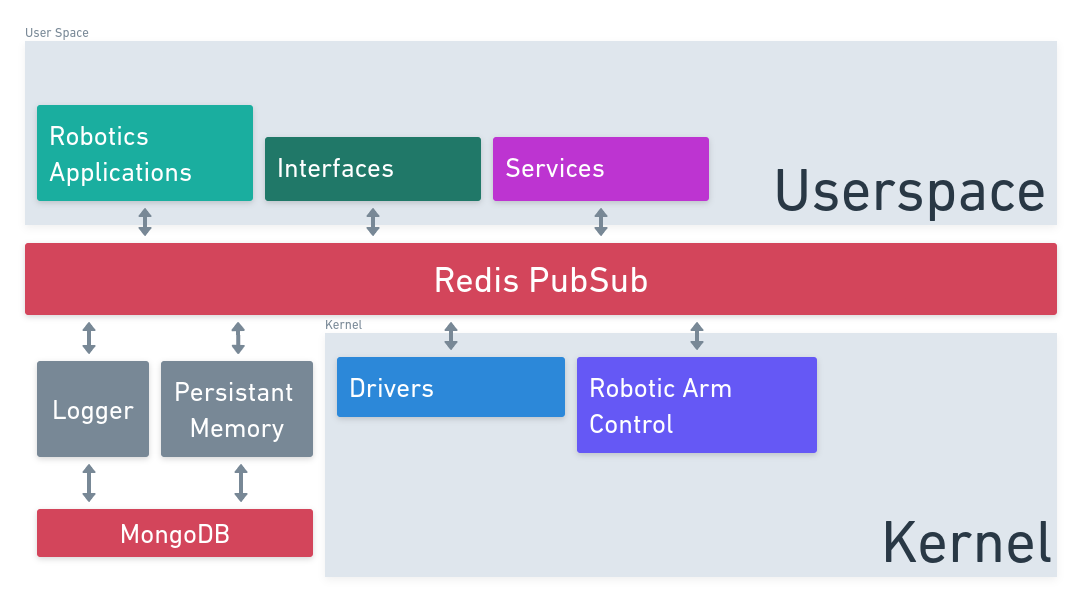
\includegraphics{images/ALFRED_arch_simple.png}
  \caption{ALFRED's architecture}
  \label{fig:arch_simple}
\end{figure}

The middleware runs in Docker \cite{docker} and is deployed with Docker Compose \cite{docker-compose}. Each component is deployed as a separate container. Using containers to deploy our software makes it easier to separate the different parts of the system but also handle dependencies. Networks\sidenote{Networks are part of Docker and enable containers to communicate with each other whereas they would normally be isolated.} are used to enable communication between components selectively. We use environment variables to configure global behavior at runtime, e.g. if the real arm should move or not.

\paragraph{Kernel}

The Kernel is the core of the middleware. It has complete control over the robot arm. It contains a Hardware Abstraction Layer (which we call the drivers) and the robotic arm control software. Drivers are the interface between external devices, such as cameras, and the Kernel. They can get data from and send commands to the devices. On the other hand, the Robotic arm control component contains the \gls{api} for moving the robotic arm, as well as utilities to manage its state (starting, stopping, handling disconnections\dots).

\paragraph{Userspace}

Userspace contains user-created components. To house user-created software, we developed the Robotics Applications Component (RAC), the interfaces and the services. The RAC contains applications, which are pieces of software that interact with the arm and implement the functionalities. Applications are modular: they can be developed outside of our middleware and integrated later with minimal changes thanks to a plug-and-play structure. Interfaces are ways to visualize what is happening in the system and interact with it in a user-friendly way. Services are components that are used to compute data but do not interact with the arm, like deep learning algorithms. They can also be used by multiple applications.

\paragraph{Inter-component communication}

Components communicate with each other using a \gls{pubsub} messaging system. This component sits between Kernel and Userspace and prevents them from interacting directly with each other. Instead, all communication has to go through the \gls{pubsub}. It provides a clear separation between Kernel and Userspace, and is our implementation of \glspl{os_ring}, or hardware access restriction. The Kernel is at ring 0 (no restrictions, most privileged) and Userspace at ring 1 (more restrictions, less privileged).




\section{Kernel}


\subsection{Related work}

\subsubsection{Robotic arm control}

Most robotic arms have an API exposing functions that allow users to control the arm more easily. Instead of controlling each of the arm's motors individually, the API exposes functions to execute complex movements, such as moving the arm to a certain position in space in a straight line, or drawing a curve from one point to the other with a certain radius.

Internally, the robotic arm's controller still translates user commands into individual motor movements. Most robotic arms provide a way for experienced developers to send these individual motor movements directly to the arm, thus reducing the load on the onboard controller. These movements can be obtained manually via mathematics, but software like PyBullet\cite{pybullet} or MATLAB\cite{MATLAB} makes it easier. They provide utilities to specify robot-specific parameters, like the number of degrees of freedom and the length of the links between the motors, from existing data. Without these tools, the programmer would have to compute these parameters themselves. They can also provide access to simulation, creating a digital copy of the robotic arm to predict behavior ahead of time.

\subsubsection{Drivers}

In the Linux kernel, drivers are implemented as modules which can be added or removed. They are written in C or Assembly for low level control over the hardware, and they expose a file which presents the data from the hardware once it has been acquired and treated. Each driver exposes a set of functions which can be called to generate data or interact with the device.

In ROS, drivers are implemented as packages, like any other software piece, that produce data to a topic. These drivers are one or more layers above the raw hardware drivers of the Linux kernel. They often use libraries which read from the device files and expose this data in a more readable format. ROS drivers are flexible in that they don't need to stream all the data all the time; instead, they can be made to output data only when something significant happens, like when a spike of current is detected from a sensor, so they can arbitrarily abstract the data for the target software.


\subsection{Robotic arm control}

The Robotic arm control component is implemented in Python 3.9 and is deployed as a container. The component is tasked with receiving commands and data from the whole system and moving the robotic arm. Its algorithm is described in \ref{alg:controller}.

\begin{algorithm}
  \caption{Robotic arm control}
  \label{alg:controller}
  \While{true}{
    $message\leftarrow$ message from pub/sub\;
    \If{$message$ is not empty}{
      parse $message$\;
      \If{$message$ is a command}{
        execute $message$ on robot arm\;
      }
      \ElseIf{$message$ is data}{
        save and use $message$\;
      }
    }
  }
\end{algorithm}


\subsection{Drivers}

Drivers are implemented in Python 3.9 and are deployed as a container. The container has full access to the host machine's hardware to be able to read and manipulate external devices. In the container, each driver is started as a background process, allowing it to run concurrently with the other drivers. When every driver is started, the parent process runs an infinite loop to keep the drivers running. Drivers have two main components: the \lstinline{DataProducer} and the \lstinline{CommandGetter}, which are started as threads and run indefinitely. They communicate with the rest of the system via the \gls{pubsub}. Topics used by the drivers have a special nomenclature, which is \lstinline{device-data-<device name>} for the \lstinline{DataProducer} and \lstinline{device-command-<device name>} for the \lstinline{CommandGetter}. Here are the algorithms for the \lstinline{CommandGetter} \ref{alg:command_getter} and the \lstinline{DataProducer} \ref{alg:data_producer}:

\begin{algorithm}
  \caption{CommandGetter}
  \label{alg:command_getter}
  \KwData{$topic\leftarrow$ "device-command-<device name>"}
  \While{true}{
    $command\leftarrow$ command from pubsub\;
    \If{$command$ is not empty}{
      parse $command$\;
      send $command$ to device\;
    }
  }
\end{algorithm}

\begin{algorithm}
  \caption{DataProducer}
  \label{alg:data_producer}
  $topic\leftarrow$ "device-data-<device name>"\;
  \While{true}{
    $data\leftarrow$ data from device\;
    \If{$data$ is not empty}{
      publish $data$ to $topic$\;
    }
  }
\end{algorithm}

Currently, drivers are implemented for these devices:
\begin{itemize}
  \item Realsense D435 cameras
  \item BLTouch sensors with a microcontroller as an intermediary data via Serial communication
  \item Microphones
\end{itemize}

The behavior of the drivers can be customized by environment variables set in the Docker Compose file.



\section{Userspace}


\subsection{Related work}

\subsubsection{Robotics applications}

In ROS, applications can be launched via the command line, but also programmatically using the roslaunch API. This requires to create a launch file specifying parameters for the application.

Outside of ROS, programs often expose APIs to make interaction possible. These API use protocols to structure communication, mainly REST (Representational State Transfer) and RPC (Remote Procedure Call). RPC is suited to executing applications from outside but has limited compatibility with the web. Thus, we considered three REST API frameworks from Python:

\begin{itemize}
  \item Flask
  \item Django
  \item FastAPI
\end{itemize}

Flask is a minimal web framework which contains basic features such as routing, debug and static files.

Django is a more heavyweight framework for creating complex websites with an SQL database as its centerpoint. It follows the Model-View-Controller pattern and has many features including an auto-generated admin panel.

FastAPI is a web framework built on top of Starlette, an ASGI (Asynchronous Server Gateway Interface) framework/toolkit. FastAPI has all the features of Flask with added functionality, such as OpenAPI docs generation and async support.


\subsection{Robotics applications}

The robotics applications component (RAC) is implemented in Python 3.9 and is deployed as a container. The RAC gives access to the robotic arm control component to the user. The RAC and the robotic arm control component communicate with each other via the \Gls{pubsub}. The API uses FastAPI \cite{fastapi} as its main technology. The RAC contains the applications which implement functionality on the robot arm. Applications can be called or interacted with via HTTP requests. To manage applications within the software, we created a class called \lstinline{Apps} class, which is a subclass of Python's \lstinline{multiprocessing.Process}. The \lstinline{Apps} class provides utilities to start applications, check if they are running, handle exceptions and provide two way communication between the application and the RAC.

Applications are managed by the RAC's \lstinline{ContextManager}, which is tasked with starting and stopping apps. The \lstinline{ContextManager} only allows for one application to run at a time, to avoid conflicts if two applications wanted to move the robotic arm at the same time.

Applications are separate processes with their own separate memory, instead of threads that share their memory with their parent. This helps avoid errors with memory management, and bypasses the restrictions of some libraries used, e.g. OpenCV not being able to show windows in anything other than the main thread.

Applications can be developed outside of our middleware and later integrated thanks to the structure of the RAC \ref{fig:api_file_structure}: applications are kept separate from the rest of the API, and live side by side. To expose an application, a route\sidenote{HTTP method (\lstinline{GET}, \lstinline{POST}, ...), path (ex: \lstinline{/applications/grasping}), and handler combination.} needs to be created. The route is then added to the applications router\sidenote{Part of the software that determines which route receives a specific request.} which is itself added to the main router.

\begin{figure}[h]
  \centering
  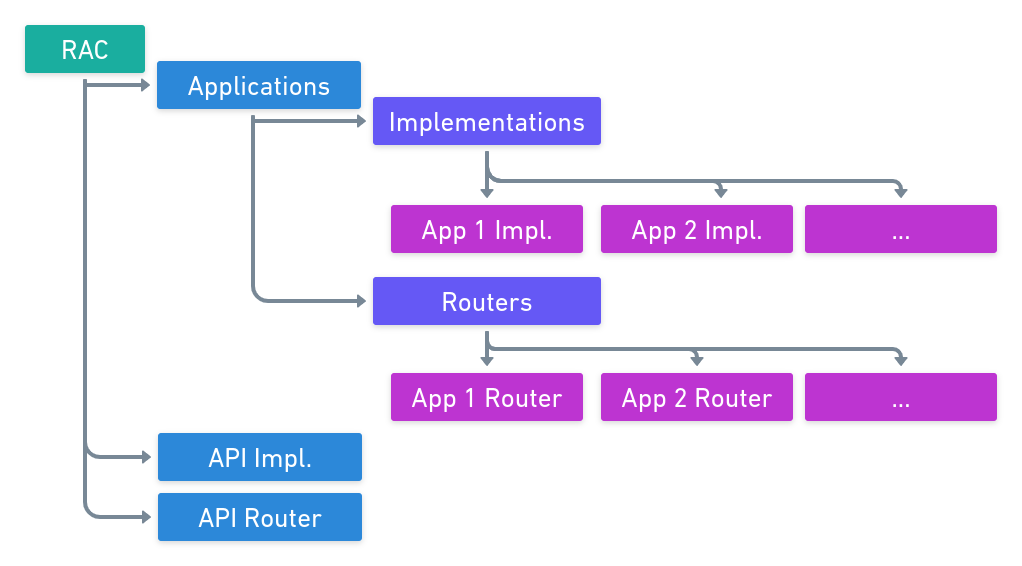
\includegraphics{images/API_file_structure.png}
  \caption{File structure of the RAC (simplified)}
  \label{fig:api_file_structure}
\end{figure}


\subsubsection{Evaluation}

Students were tasked with developing applications using ALFRED.
One of them created a driver for a BLTouch bed leveling device interfaced with a micro-controller, and an application using this device to create a 3D map of any mostly flat surface.
Another created an interface plugging into the middleware to act as a dashboard, showing system information and executing applications.
Here were their remarks about the system:

\begin{itemize}
  \item The application was able to be developed outside of the middleware and then integrated with minimal changes, in less than a day.
  \item Creating the application didn't require extensive knowledge about robotics or the robot arm.
  \item The driver was conceived with few (about 30 added) lines of code from a basic template.
  \item The data exposed by the RAC allowed the dashboard to show meaningful system data such as the current position of the robot.
  \item The dashboard was able to be developed outside of the system and then integrated only by setting up the appropriate Docker environment.
\end{itemize}


\subsection{Services}

Services are implemented as Docker containers. Since they are a bit more generic, the user is responsible for specifying the dependencies for their services in the component's \lstinline{Dockerfile}. Examples for services are a Natural Language Processing server or an API for external programs such as Unity. We separated services from robotics applications because some services could require different versions of Python, or even a completely different runtime environment. At the moment, services have to be added manually into the whole middleware's Docker Compose file.


\subsection{Human-Robot Interfaces}

Interfaces are a type of service meant to handle input and output from the user. An example of interface is a Web dashboard for viewing the status of the system and managing applications.



\section{Inter-component communication}


\subsection{Related work}

Message handling can be done with ROS via its topics. Messages can be sent by pieces of software to a specific topic, and other pieces of software can subscribe to topics to get the messages. Messages are defined by a \lstinline{type} which defines the structure of the message and allows ROS to automatically parse messages.

Redis is another solution for realtime communication between processes, specifically its \Gls{pubsub} module. Redis Pub/Sub uses channels where publishers can push data and subscriber can subscribe to get data. Messages don't have types which means the publisher is responsible for encoding the data and the subscriber is responsible for decoding it but the communication was found to be faster than ROS \cite{redis_benchmark}.

Other solutions for inter-process communication include D-Bus. D-Bus is based around a message bus daemon which applications connect to. Applications use a library, libdbus, to interact with the message bus. The daemon acts as a router, sending messages from one application to another. Communication is one-to-one only.


\subsection{Communication bus}

Inter-component communication is done with Redis \cite{redis}, specifically Redis' \Gls{pubsub} implementation. It runs in a Docker container from the Bitnami image, \lstinline{bitnami/redis} version 7.0 with default settings. The \Gls{pubsub} sits in-between the Kernel and Userspace and allows components to send each other data.


\subsection{Persistent storage}

The Redis Pub/Sub doesn't persist the data it receives to disk, so MongoDB is used for long-term storage. Data stored includes logs and component-specific data, but it can also serve as a way to save messages sent via the \Gls{pubsub}. The Kernel possesses its own database for storing system-critical data, while the data from the Userspace database can be accessed by both Userspace and Kernel.



\section{Conclusion}


\subsection{Applications}

In this chapter, we described an infrastructure for developing applications on robotic arms. It follows the architecture of UNIX-like operating systems with its separation into Kernel and Userspace and the associated \glspl{os_ring} to define privileges.

This middleware makes developing robotics applications accessible to users with limited knowledge about robotics and robotic arms. It means that developers need less training and that they can have more confidence that their software won't cause damage on the system.

Thanks to its modular architecture, software can be created outside of the system and integrated later with minimal modifications. This is useful since debugging becomes harder the more complex a system is. With isolated software, developers can find and fix issues more rapidly.

With the use of a central \Gls{pubsub} messaging system, components don't need to know who they are sending their data to, but only need to determine the name of a channel that the relevant software can listen on. With this, we can reduce how strongly components depend on each other, which is called coupling. Reduced coupling makes breaking changes less frequent when modifying related code since the components communicating are not directly linked to each other.


\subsection{Limitations}

Running every component as Docker containers adds a complexity that would not exist with native execution. The robotics applications component still has to be run in \lstinline{privileged} mode\sidenote{Privileged: has access to every device. Unprivileged: cannot use the host computer's devices.}, because some applications require access to the screen to show information. Running in \lstinline{privileged} mode diminishes the usefulness of having a separation between Kernel and Userspace, since in the end Userspace can still access devices directly.

Running in Docker also means components are difficult to debug once they have been integrated into the system. This is because every time a modification has to be done, the system needs to be stopped, built, and then started again for the changes to be taken into account. Approximate times are shown in table \ref{table:restart_times_docker}. Build times can be especially long when dependencies are changed and the whole image has to be rebuilt. Setup times can also be long depending on the applications, e.g. when loading a deep learning model. Such long restart times decrease the efficiency at which the project can be iterated on.

\begin{table}[ht]
  \centering
  \caption{System restart times.}
  \label{table:restart_times_docker}
  \begin{tabular}[t]{lcc}
    \hline
                  & Time (best, seconds) & Time (worst, seconds) \\
    \hline
    Stop      & 20           & 30           \\
    Build     & 20           & 600+         \\
    Start     & 20           & 30           \\
    Setup     & 10           & 300+         \\
    \hline
    Total     & 70           & 960+         \\
    \hline
  \end{tabular}
\end{table}%

As it is, the controller is using ALFRED's specific robot arm's API to move the arm.
This means that applications developed for this specific robotic arm will not be compatible on another arm.
It also means that the control of the finite movements of the robotic arm comes from an external program, and so the middleware's controller component can't directly influence said control.


\subsection{Future works}

Issues with the API running in \lstinline{privileged} mode can be solved by delegating the responsibility of showing information to the Kernel. An interface could be implemented to get image buffers from applications in Userspace and then show these image buffers on screen. Options for configuration would need to be added to respond to the needs of applications in terms of interface. Also, since window controls would be under ownership of the Kernel, applications wouldn't be able to capture user input by themselves, so the Kernel would need to pass these inputs through to the applications.

Some methods were used during development to reduce restart times, but they are not properly integrated and impractical to use by the general public. We plan on creating a fully integrated \lstinline{dev} mode for the system. \lstinline{Dev} mode would enable programmers to make changes without having to rebuild the whole system. This mode would add a feature to automatically reload the Docker container's program(s) when a file is changed or upon user request. Files in the host computer would need to be synchronized with the files inside of the containers, which can be done with Docker \lstinline{volumes}.

As they are implemented currently, services and interfaces are not very well integrated into the system. Indeed, the user has to create their Docker image on their own, add it to the main Compose file, and configure it properly. We want to make services and interfaces easier to add to the system by automating the discovery and integration of services into ALFRED. This piece of software would expose utilities to add new entries in the main Compose file securely with a template. It would allow experienced users to provide their own Docker images, program files, and configuration manually, and less experienced users to use common configurations to quickly and easily deploy new services.

We plan on generalizing the middleware for every robotic arm. To do so, we could first create a mapping between our generalized API for robotic movement and the associated function for every robotic arm. This would change the function that is called within robotic arm control depending on the model of the robotic arm used, but wouldn't change the function called in Userspace. Later, we would step away from using the robotic arms' APIs, and compute the robot's movements ourselves using Inverse Kinematics, only sending motor movements to the robotic arms.

    % \chapter{Human-robot interaction}



\section{Introduction}

As robotic arms evolved from specialized operators capable of only executing a single task to complex structures with high computing power, humans became able to interact more closely with the machines.

Human-robot interaction (HRI) studies the means of communication between humans and robots by designing, understanding, and evaluating robotic systems that coexist with humans. It is a multidisciplinary field with contributions from human-computer interaction, artificial intelligence, robotics, natural-language understanding, design, and psychology.

Interaction can be separated into two general categories: remote and proximate. In remote interaction, the human and the robot are separated spatially, or even possibly temporally. Remote interaction can be \lstinline{teleoperation} if the robot is controlled by its interaction with the human as a general supervisor, or \lstinline{telemanipulation} if the human controls the robot completely via a physical manipulator.

In proximate interaction, communication is often more social, focusing on more abstract concepts such as emotions. The robot can perceive the human with sensibility to touch, for physical interaction; sight, for analyzing posture and facial signals; or hearing and speaking to communicate verbally like a real human.

We designed two interfaces for remote and proximate interaction. First, hand movement and gesture control, which allows the human to manipulate the robotic arm remotely by using their hand as a guide for the robot and making hand gestures to trigger actions. And second, voice control, a proximate interaction using natural language understanding to enable the robot to accept commands formulated in a natural, "human-like" manner.



\section{Related work}

Many technologies can be used to develop interactions due to the flexible nature of robotic platforms. From computer vision, to wearable electronics, to virtual reality, many things can be adapted to enable control of a robotic arm.

Using a Virtual Reality headset, Lipton et al. \cite{robot_control_vr} were able to create a platform for teleoperation, implementing tasks such as pick and place, assembly, and manufacturing. It takes inspiration from Penfield's Homunculus model \cite{penfield1950cerebral}, creating a mapping from human to robot enhancing sight and hand feeling.

Complete structures can also be constructed to place the user in a sort of "command chair", where they can precisely move the robot \cite{centauro} \ref{fig:centauro}.

\begin{marginfigure}
    \centering
    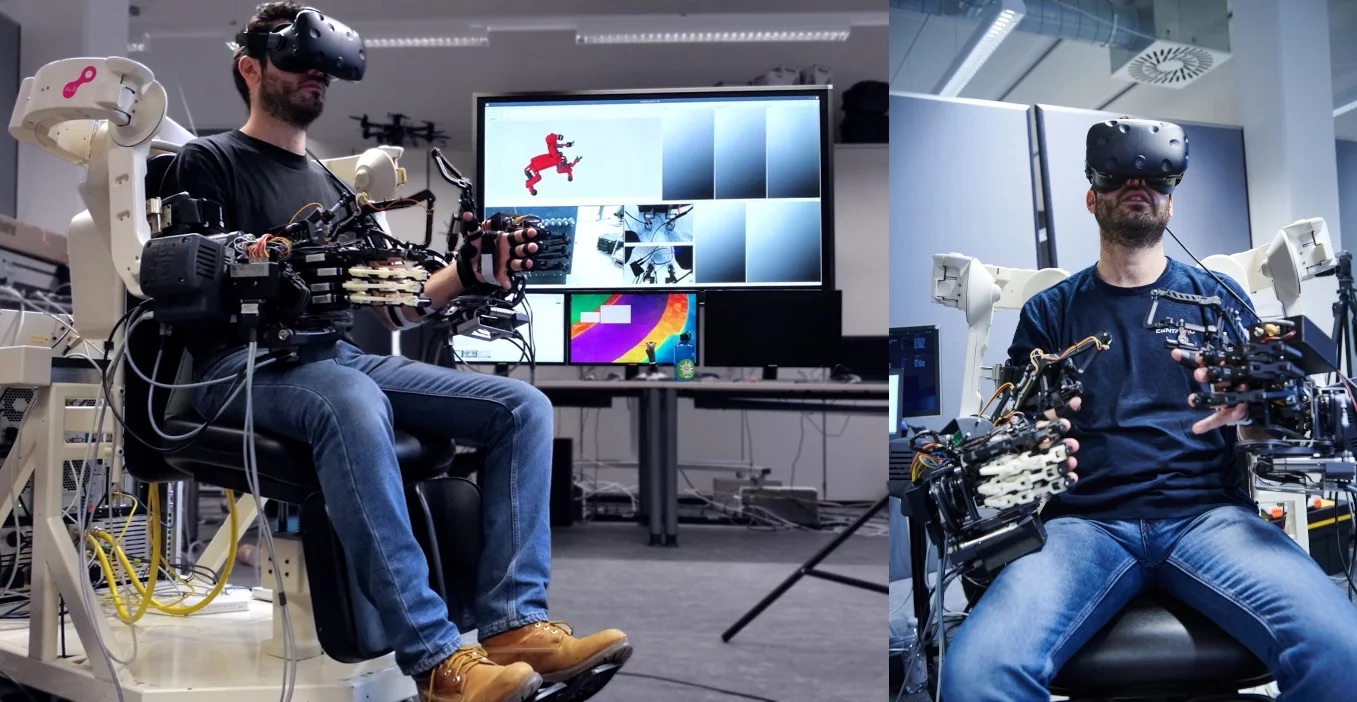
\includegraphics{images/centauro.png}
    \caption{Centauro project control chair}
    \label{fig:centauro}
\end{marginfigure}

To create a direct link between the robot brain and the human brain, Salazar-Gomez et al. \cite{robot_control_eeg} use an EEG (Electroencephalogram) headset to detect brain signals related to unexpected error making (ErrPs) to correct mistakes in classification tasks. It can change the behavior of a robotic arm when it is making a mistake during a task consisting of sorting object into different labelled bins.

The body itself can act as a control interface using wearable devices \cite{robot_gesture_control_wearable}. By measuring biceps, triceps and forearm activity, but also arm motion, DelPreto et al. were able to control a drone through obstacles using only their arm.

Interfaces can be used to explore the relationships between human and robot. By studying the emotional response of humans giving an object to a robot, and the robot taking the object in different manners, we can, for example, find the characteristics of robotic movements that make them more trustworthy in the eyes of humans, to make them more socially apt, and to mimic human-human interactions \cite{robot_handoff}.

There are also ways of controlling a robot that don't involve physical contact or devices. Matarneh et al. \cite{matarneh_maksymova_deineko_lyashenko_1970} used a deep learning algorithm, specifically a multi-layer perceptron, to interpret voice into commands. With these commands, researchers were able to control the movements of the robot directly from voice data, while other solutions involve translating voice into text first, and then text into commands \cite{Janicek_2021}.



\section{Hand movement and gesture control}


\subsection{Introduction}

A robotic arm closely mimics the workings of the human arm, with joints and muscles in the form of motors. It is not surprising, then, that we would want to create a link between the human arm and the robot arm. On another level, grasping tasks are some of the most common tasks of a robotic arm, just like the hand of the human.

These are the reasons why we created hand movement and gesture control for ALFRED. By mirroring the robot and human arms, we can create a strong connection between machine and operator. We can take advantage of the dexterity of the hand and translate this dexterity into the robotic arm by interpreting complex hand gestures into commands for the robot. Hand movement and gesture control can be used as a remote interface, making the robotic arm act as the user's arm in another place, or as a proximate interface, acting like a mirror showing a robotic image of the user to aid them in their current task.


% \subsection{Related work}

% % XXX: related_work


\subsection{Contribution}

\subsubsection{Concept}

\begin{figure}[h]
    \centering
    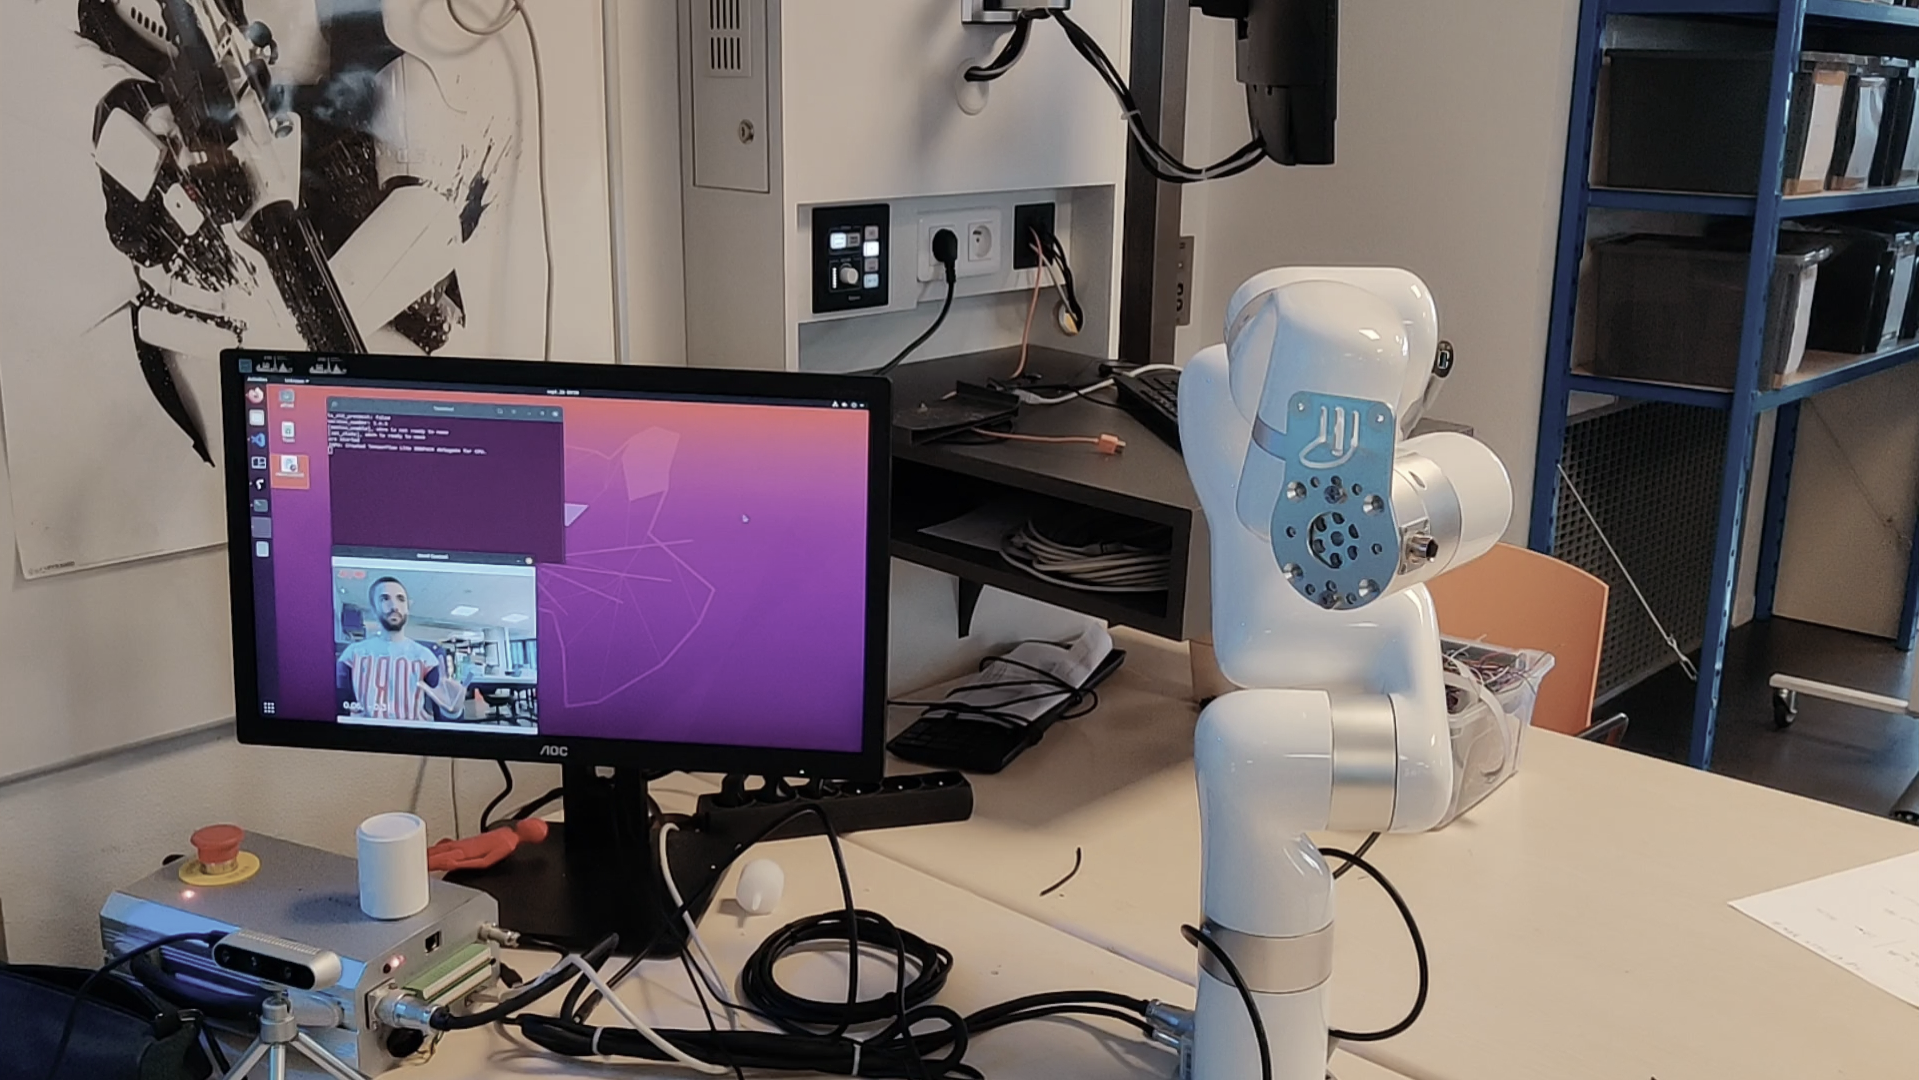
\includegraphics{images/hand_control_overview.png}
    \caption{Operating the arm with hand control. On the left, the computer running ALFRED with a camera pointed at the operator, showing the annotated camera feed. On the left, the robotic arm being controlled.}
    \label{fig:hand_control_overview}
\end{figure}

Hand control allows an operator to control the robotic arm with their hands \ref{fig:hand_control_overview}. It uses a camera pointed towards the operator and a hand recognition algorithm to detect the position of the hand. It then interprets the data to control the robotic arm. The hand control interface moves the robotic arm by comparing the position of the center of the hand\sidenote{Taken as the middle of the segment between the wrist and the index finger metacarpal} to the center of the video frame. If the hand is on the left of the center of the frame, the robot will move left (as seen from the front). The further away from the center the hand is, the faster the robot moves.

We trained machine and deep learning models to detect gestures which allow for further interaction, such as opening and closing a gripper, or starting and stopping other applications.

\subsubsection{Implementation}

Hand control has been implemented following the principle of dependency injection. The software contains only video processing, while video acquisition and moving the robotic arm itself are left to system developers. This allows modularity and adaptability for many, if not all, systems. In ALFRED, video acquisition is done through the drivers with a stream from the Pub/Sub abstracted by a class. Moving the robotic arm is done through a function injected into the Hand control software. The function takes in landmarks and gesture data from the model and translated them to robot commands specific to the robotic arm.

For the processing part itself, Hand control uses video frame data, hand detection, and post-processing to transform hand position into robotic arm commands. From frame data, hand detection is run using Mediapipe Hands\cite{mediapipe_hands}.

We extract 3D landmarks which represent the various points of interest on the hand. These landmarks represent the wrist and each finger joint, as well as each finger tip, for a total of 21 landmarks.

Two models were built to detect gestures from the landmarks. We built a dataset of hand gestures and their corresponding landmarks. The data was collected by taking a video of a subject doing the same hand gesture for a couple of seconds, moving and rotating their hand constantly and randomly. We only recorded the landmarks instead of the whole frames, so we only had 42 (21 landmarks, and x and y values for each landmark) values to record instead of the 640x480x3 values of the RGB frame. The data was augmented with small random rotations, as well as mirroring to enable generalization for both hands. We then trained a Random Forest using scikit-learn\cite{scikit-learn}, and a Multilayer Perceptron (MLP) implemented in PyTorch, with a few layers activated by the ReLU function.

From the hand landmarks, we create robot commands. Our initial command method was to create a linear mapping between the position of the hand and that of the robot's end effector. User feedback allowed us to finetune the method to be more intuitive and capable. This second method mimics the working of game controller joysticks. We transform the camera fram into the joystick: when the user moves their hand to the left of the frame, the robot moves continuously to the left. The speed of the movement is dependent on the distance between the center of the hand and the center of the frame.

The center of the frame contains a dead zone a couple of pixels in radius. When the user places their hand in this zone, no movement command will be issued. Gesture commands can still be recognized and issued. This was found to be necessary because the arm would make small movements when the user didn't want it to move. It would also add latency to the next movements: robot commands would be queued continuously and clog up the command queue.

To implement this control method, we compare the center of the hand to the center of the frame, and multiply the difference by an offset, found empirically (in our case, it is \lstinline{0.022}). The commands are then sent to move the robotic arm. The two methods are illustrated here \ref{fig:hand_control_methods}.

\begin{figure}
    \centering
    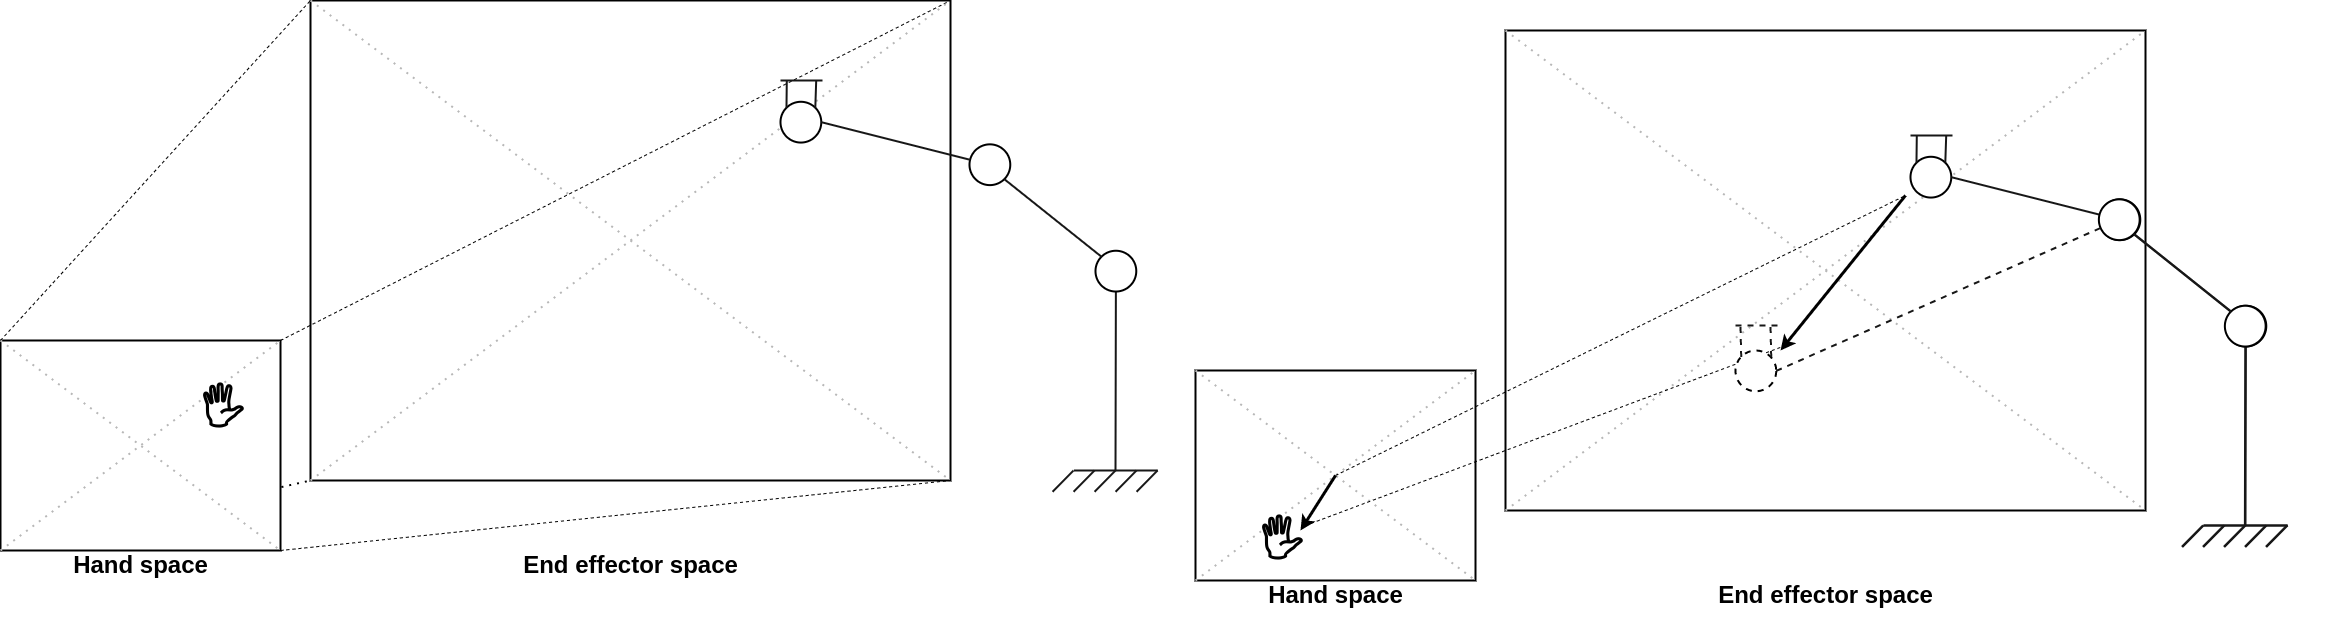
\includegraphics{images/hand_control_methods.png}
    \caption{First (left) and second (right) methods for translating hand position to robot command.}
    \label{fig:hand_control_methods}
\end{figure}


\subsubsection{Evaluation}

The goal of this interaction was to create a way to control a robotic arm that would be more intuitive than using gauges and dials on a computer screen. We selected four criteria to measure its effectiveness:

\begin{itemize}
    \item Intuitiveness: how natural it feels
    \item Usability: how good it feels to use
    \item Mobility: how it can move in its environment
    \item Precision: how difficult small movements are to achieve
\end{itemize}

We asked 8 participants to test the interaction. Of the 8, 5 had prior knowledge of the system and had at least a basic understanding of robotics, while the rest had no prior knowledge and no knowledge of robotics.

We used two tasks to evaluate our interaction:

\begin{itemize}
    \item Free exploration (intuitiveness, usability, mobility)
    \item Moving a plastic can balanced on top of a piece of wood (precision) \ref{fig:hand_control_task}
\end{itemize}

\begin{figure}[h]
    \centering
    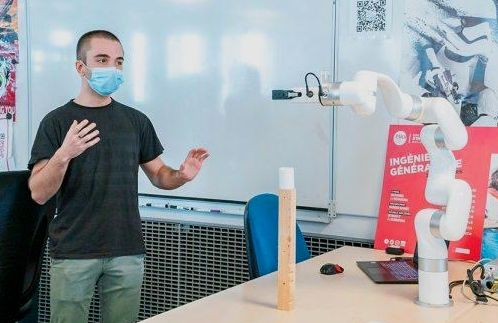
\includegraphics{images/hand_control_grasping.jpg}
    \caption{Preparing to grab the piece of wood to move the plastic can}
    \label{fig:hand_control_task}
\end{figure}

Free exploration was overall appreciated by the participants. It took them about five minutes to understand how the system works, which we found to be acceptable. Six out of the eight found the chosen method to be intuitive, and all the participants found it to be an effective method. There was one problem when starting the control session, specifically with the initial hand pose: the hand had to be perfectly centered or else the software would send the robot commands when it was still setting up, resulting in erratic movements that would sometimes break the system. Once aware of this problem, participants were able to avoid it reliably. The most limiting factor was range of motion, where the arm would make very big and fast movements when approaching the end of its operating zone. This would oftentimes break the software which would require a reboot. We can therefore validate intuitiveness and usability, but there needs to be further work on mobility by making further regions safer to operate in.

Our precision task used gestures, namely closing and opening the hand, to grab and release with the gripper robotic arm's gripper. The objective was to pick up and move a piece of wood with a 3D-printed soda can balanced on it in a circle, then put it back down. Four participants, all with prior knowledge, managed to complete the task, while the other four failed. Of the four that failed, two did because the gripper released the piece of wood too early, causing it to drop to the table. From this experiment, we can conclude that precision tasks required more trained operators, and that we had to improve the reliability of the system, specifically with hand gestures.


\subsection{Conclusion}

\subsubsection{Applications and use cases}

Hand movement and gesture control can be applied to any robotic arm to allow a minimally-trained operator to control the arm.

With this more natural method of control, as opposed to moving a slider or clicking on arrows, operators are able to achieve higher precision and a stronger connection between them and the robot.

More precise control for minimally trained operators means Hand movement and gesture control can be used by factory workers to move heavy weights, for example in a construction of metal factory, with a bigger industrial arm. It can also be used by researchers in laboratories, for moving dangerous pieces of equipment or chemicals during an experiment where hand manipulation, even through a glove box, would be risky. Finally, given the appropriate equipment, we could imagine a robotic arm moving through rough and dangerous terrain in rescue or cleanup operations.

\subsubsection{Limitations}

The main limitation for Hand movement and gesture control currently is the dimensionality: the arm can only be made to move in a plane. It cannot move in three dimensions which severely reduces its capabilities. Even more importantly, there is no way to rotate the arm. It will always be facing in the same orientation.

Secondly, using such a simple interface as the hand means that more advanced controls need to be hidden behind certain commands, or in our case gestures. This increases the complexity for understanding the system.

\subsubsection{Future works}

In the future, we would like to improve the system on the problems found in the user study and alleviate one of the limitations.

Mobility would be improved by creating safeguards around the edged of the range of motion to create smoother movements around these edges. Range of motion would be reduced a bit but to the benefit of more system reliability and easier handling because the system would not break or create sudden unplanned movements.

Grabbing reliability, or more generally gesture handling reliability, also needs improvement. Systems can be put in place to avoid suddenly releasing a grabbed object because of an error in gesture detection. For example, with buffering and outlier removal.

Another main aspect that would be improved is the dimensionality. While the arm can currently only be made to move in two dimensions (in a plane) with Hand movement control, we would like to make it move in three dimensions. This could be done by using depth frame data to measure the proximity of the hand to the camera. With some calibration at the beginning of handling, we could detect wether the operator moves their hand backwards or forwards, creating the possibility for the arm to move in the three dimensions.



\section{Vocal command control}


\subsection{Introduction}

Recent years have seen the rise of home assistants such as Siri from Apple or Alexa from Amazon. These assistants use complex deep learning algorithms to interpret the sound of your voice into commands to execute. These devices allow their users to control their home and automate tasks without having to touch anything. They act like a butler, constantly listening for requests and executing them when received.

We wanted to reproduce the same functionality for ALFRED: to allow users to talk to the platform as a means of interaction. Like home assistants, the objective was to create a "butler" that listens, like a human, to commands expressed in natural language, instead of pre-defined sentences. It would thus be more integrated into its environment as something almost living and intelligent.


% \subsection{Related work}

% % XXX: related_work


\subsection{Contribution}

\subsubsection{Concept}

Voice control allows an operator to control the robotic arm vocally. With data from the microphone driver, a Speech Recognition algorithm interprets the voice into text (Speech-To-Text, or STT). Text data is then interpreted by a Natural Language Processing (NLP) algorithm to extract intent and data from the command. From the intent, the system determines which API function to call, also sending the extracted data when necessary.

\subsubsection{Implementation}

We built a driver for microphones which provides raw audio data but is also capable of doing Speech-To-Text (STT). Using Azure Speech \cite{azure_speech}, we convert raw sound data (also from the driver) into text. We do continuous speech recognition: the STT model recognizes each word as it is spoken, and combines words together when a pause indicating the end of the sentence is detected. At the moment, only complete phrases are sent by the driver.

With the sentences detected by the STT part of the microphone driver, we run an NLP algorithm. Voice control uses RASA\cite{rasa}, a machine learning framework for building automation around text conversations. It uses Natural Language Understanding (NLU) to process text into intents and variables, which we call command data.

Intents are the purpose behind the sentence that was treated. Currently implemented intents include:

\begin{itemize}
    \item \lstinline{call}: Activate listening. Unless the system is called, it will not respond to commands, to avoid doing everything it hears against the operator's consent. Listening stays activated for a short period of time or until it is manually deactivated. An example of a sentence for this intent is: "Hey Alfred".
    \item \lstinline{uncall}: Deactivate listening. An example is: "Thank you Alfred".
    \item \lstinline{grab_object}: Grab the specified object. An example is: "Can you grab the cup ?"
    \item \lstinline{call+grab_object}: Associates the \lstinline{call} and \lstinline{grab_object} intents. An example is: "Hey Alfred, grab the bottle please".
\end{itemize}

Command data is a word or a set of words extracted from the command, that can change for the same intent. In the case of grabbing objects, data would be the object to grab. For example, in "Grab the pen please", RASA would extract the intent as "grab" and the data as "pen".

From the intent, the system determines which API function to call, also sending the extracted data when necessary.

% \subsubsection{Evaluation}


\subsection{Conclusion}

\subsubsection{Applications and use cases}

Voice control is used within ALFRED to interact with the system vocally. It allows users to manipulate the system in a natural manner, like talking to a human assistant. Voice control can also be integrated in other systems to make them controllable by voice. API routes can be mapped to voice control intents to make the system more accessible to users, in line with the objective of seamless integration.

Its applications can be imagined in makerspaces, as an interface for an automated personal assistant. The user could be doing a manual task and direct the assistant with their voice, in a natural manner. The user wouldn't need to put down their equipment to manipulate the assistant, and instead could continue doing their task in a seamless manner.

It could assist people who can't move their arms because of a disability who would have trouble controlling the robotic arm with a mouse and keyboard, or a controller, or even Hand and gesture control.

\subsubsection{Limitations}

Voice control is held back by its training complexity. Due to the nature of the software used, voice control cannot generalize easily for new commands or conversation paths. Each new intent needs dozens of training samples which need to be carefully selected, and each time the model must be re-trained and re-deployed. This makes it difficult for developers to extend Voice control with their specific use cases.

\subsubsection{Future works}

More intents and stories need to be developed to enable the Voice control software to be an autonomous assistant. Currently, it can only call functions from the robotics platform, but the goal is to make it more of an interface that can show the full capabilities of the platform, from listing all available features to describing the current state of the platform, or even to make tutorials and demonstrate how to do certain tasks with or without the robotic arm.



\section{Conclusion}

One of our objectives with ALFRED is to allow people to design interactions with a robotic arm and to provide the tools to facilitate doing so.

We explored the possibilities of ALFRED by creating two interactions of our own: hand movement and gesture control, and voice control. These interactions allowed us to finetune our system to make it more usable by future developers. When designing the interactions, we created services to enable the creation of the RASA server, a software unit that was not a driver, but also not a robotic application.

We discovered the idea of creating a connection between man and robot by mapping body parts to the robotic arm, and we searched for ways of translating body movements into robot commands that would feel natural to us humans.

Finally, deep learning was used to transform a simple robotic arm into a smart assistant and an integral part of the space it is located in.

    % \chapter{Robotics applications}



\section{Introduction}

The actions a robotic arm can take decide its usefulness. To assist a person in their everyday lives, the arm should be able to, among other things, manipulate objects or interact with machines. To assist in an industrial context, it must be able to use the tools necessary for the task and to be reliable.

What we call applications within ALFRED are the pieces of software that implement the possible actions of the robotic arm. As we presented in a prior chapter, they live in the Userspace where any user is free to implement their applications for their use cases.

We present two applications that were developed to add capabilities to the robotics platform: writing and drawing, and object grasping and manipulation.



% \section{Related work}

% TODO (main related works section)

% \cite{mit_rfusion}
% \marginfig{mit_rfid}

% \cite{quayola_sculpture}
% \marginfig{robot_sculpture}



\section{Writing and drawing}


\subsection{Introduction}

Writing is a complex motor task that children take years to do properly. Drawing is even more complicated, and becoming an artist capable of expressing their thoughts in paper or a digital format is a lifelong endeavor.

A robot can learn these skills by learning the movements once without needing time to practice. Writing and drawing can be useful in automation, where a factory would want to create custom handwritten notes, or sign papers with a pen automatically. It can also help people who can't write by themselves, and don't want to, or can't, transition completely to digital media.


% \subsection{Related work}

% % XXX: related_work


\subsection{Contribution}

\subsubsection{Concept}

This application uses the robotic arm to write text autonomously. It transforms its input text into a sequence of movements of the robotic arm, thus enabling the robot to write on any flat surface, independent of orientation.

The original gripper could not grasp the pen efficiently enough to do continuous writing, so we developed a custom mount for the pen, taking advantage of the provided schematics for the arm's end effector.

% TODO: schematic of the pen mount

The system was then adapted to use the robotic arm to draw line art of images \ref{fig:writing_and_drawing}.

\begin{figure}[h]
    \centering
    
\includegraphics[height=7cm]{images/writing.png}
    \hspace{1cm}
    
\includegraphics[height=7cm]{images/drawing.png}
    \caption{Writing and drawing}
    \label{fig:writing_and_drawing}
\end{figure}

\subsubsection{Implementation}

\paragraph{Writing}

The API for the writing application takes in a string of the letters to write. It uses a mapping between letters and an array of robot instructions. These robot instructions are numbers and booleans, whose structure is adapted from the API of the robotic arm to be more comprehensible to the programmer. This structure is as follows:

\begin{itemize}
    \item 6 numbers for x, y, z, roll, pitch, yaw. These values are not interpreted as absolute movements relative to a fixed point in space but as relative to the actual position of the arm.
    \item 1 number for the radius of the movement. If the radius is 0, the movement will be a straight line. If it is bigger than 0, the movement will be a curve with the specified radius.
    \item 1 boolean to specify if the radius is in degrees or radians.
\end{itemize}

% TODO: add figure of coord space

Here is an example for the letter D:

\begin{lstlisting}[language=Python, caption=Example for the letter D]
mapping = {
# ...
    "D": [
            # Starting pen up, go to the top left corner
            [10, 0, 0, 0, 0, 0, 0, False],
            # Lower the pen to the paper
            [0, 0, 5, 0, 0, 0, 0, False],
            # Draw the left bar of the D
            [-10, 0, 0, 0, 0, 0, 0, False],
            # Raise the pen
            [0, 0, -5, 0, 0, 0, 0, False],
            # Go back to the top left corner
            [10, 0, 0, 0, 0, 0, 0, False],
            # Lower the pen again
            [0, 0, 5, 0, 0, 0, 0, False],
            # Draw the semi-circle of the D
            [0, 7, 0, 0, 0, 0, 7, False],
            [-10, 0, 0, 0, 0, 0, 7, False],
            [0, -7, 0, 0, 0, 0, 0, False],
            # Raise the pen and prepare for the next letter
            [0, 10, -5, 0, 0, 0, 0, False],
        ],
# ...
}
\end{lstlisting}

The instructions in the mapping use a relative notation, but the performance of moving with only relative motions was not sufficient for the needs of the application. It added delays from calculating the absolute position internally and the movement was choppy. To correct this issue, we store the arm's position at the beginning of each sentence and calculate the absolute position from the relative movements for each robot instruction.

\paragraph{Drawing}

Using the same system as writing as a base, we added the possibility for the arm to draw line art of images. This feature uses images in the Scalable Vector Graphics (SVG) format to extract and draw line art. Images in the SVG format are not described as a matrix of pixels, but rather a series of lines described by mathematical equations. This normally allows the images to be scaled up or down infinitely, but in our case, we use these equations as guides for the trajectory the robot should use to draw the picture.

We support a subset of the SVG format. The supported path instructions are:

\begin{itemize}
    \item MoveTo, or M: move the cursor to the specified position without writing
    \item LineTo, or L: move in a straight line
    \item CurveTo, or C: move in an arc as described by a Bezier curve
    \item ClosePath, or Z: go back to the place the cursor started writing
\end{itemize}

SVG files are pre-processed by hand to remove all unnecessary information. Only the path attributes are kept, and they are formatted to have one command per line. In code, the pre-processed file is parsed into an array containing each command in order. The commands are then translated into the same type of robot instructions as writing. For circles and lines, we first translate the command into a mathematical equation which we then sample according to a manually defined, arbitrary precision level.

This translation essentially creates the same value as the alphabet mapping, where here the key is the id of the drawing and the value is a much more complex array of robot instructions.

% \subsubsection{Evaluation}

\subsection{Conclusion}

\subsubsection{Applications and use cases}

Enabling a robotic arm to write allows anyone with such equipment to write or draw autonomously. This feature allows users to write text on paper without their hands, which can be useful for impaired users or in multitasking situations. This application can also be used to automate writing in a factory or small business. With drawing, company logos or signatures can also be automated.

\subsubsection{Limitations}

One of the drawbacks of our approach is speed. Due to the precise nature of writing, movements need to be slow or the letters produced by the arm are not well drawn, curved or slanted.

Another limitation is the complexity of the setup required. This is caused by the absence of any feedback mechanism on the pen and pen mount. The drawing surface needs to be on a perfectly flat and level surface because the pen cannot adapt itself to the surface. As an extension of this problem, careful calibration is required to make writing work. The pen needs to be placed precisely on the axis perpendicular to the drawing surface (Z-axis calibration). Too high and it will not make contact when writing, too low and it will be forced into the writing support and break. The plane of the robot end effector needs to be perfectly parallel to the plane of the writing surface, or it could progressively go away or towards the surface when writing (XY-axis calibration). This problem can be mitigated by using a large pen like a whiteboard marker and a soft writing surface, so that the pen can dig into the surface a little bit and still write, but it is not an elegant nor viable solution.

\subsubsection{Future works}

One of the possible improvements that can be done to this application is the automation of drawing. Currently, only SVG images are supported, and they have to be pre-processed manually. With edge finding and line fitting algorithms, we could transform any image into lines and then into mathematical equations that could be sampled to give robot instructions.

Another improvement would be the integration of hand writing. By mixing together drawing and writing, we could be able to interpret a user's hand writing as a drawing and use it in our alphabet mapping to replace the original simple letters by custom hand writing. This would improve the system for writing automation since the writing would be much more visually appealing. The system could then be used to automate the writing of custom sentences e.g. for notes.

Finally, to correct the limitation of the writing surface, we could integrate a bed levelling application (which was already developed on ALFRED) to find the location and orientation of the writing surface, removing the need for Z- and XY-axis calibration.



\section{Object grasping and manipulation}


\subsection{Introduction}

Robotic arms traditionally use hardware attached to their end effectors to interact with their environments. When a robotic arm is used to automate welding, for example, it will be equipped with a tool specifically made for this application.

However, in flexible environments such as homes or research laboratories, tasks are more varied than in assembly chains. Using the same approach as in factories would require tools to be changed too often, or specific tools to be made for every variation of a task or environment. Instead, by giving the robotic arm the capability to grasp and manipulate objects, we can make it adapt to many more environments and tasks.


% \subsection{Related work}

% % XXX: related work


\subsection{Contribution}

\subsubsection{Concept}

This application consists of looking for a specific object in a radius around the robotic arm and grasping it once it is found. The operator can then manipulate the object with the robotic arm through voice commands.

First, an object type has to be registered. This can be done at the application's start or during its execution. The robotic arm will then enter \lstinline{scanning mode}: in a loop, it will look at its surroundings section be section to look for the object.

When the object is detected, the application enters \lstinline{homing mode}. In homing mode, the arm centers the camera on the detected object. It starts off with big movements to get close as fast as possible, then uses smaller and smaller movements the closer it gets.

Once homed on the object, the robotic arm begins its approach for grasping. Using camera color frames, it checks that it is still centered on the object. Using camera depth frames, it detects how close it is to the object. Once it is close enough, it closes the gripper. Grasping force is estimated from the depth frames by finding the approximate size of the object. To verify the object has been grasped correctly, we look at the value of the current going to the gripper: a higher value than normal means the gripper is applying force to the object, and therefore that is has grasped it.

If the robotic arm grasped the object successfully, it can then await further commands via the voice interface. Possible commands are to move the object in a certain direction, to hand it to the operator, or to place it back on the experiment space \ref{fig:grasping_cup}.

If at any point in time the system loses the object, the arm executes its \lstinline{return sequence}, getting back into position for scanning.

\begin{figure}[h]
    \centering
    \includegraphics{images/grasping_cup.png}
    \caption{Robot arm grasping a cup, ready to accept commands for manipulation}
    \label{fig:grasping_cup}
\end{figure}

\subsubsection{Implementation}

\paragraph{Starting and interacting with the application}

At its base level, the application is called via an API route within ALFRED. The object to grasp can be given when starting the application or left blank, in which case the arm will not scan for any object. The target object can be changed during execution with another API route. Within ALFRED, applications are run as processes and therefore cannot normally be interacted with\sidenote{Contrary to threads, processes' memories are kept separate which renders memory sharing impossible and thus makes communication harder.}. We thus implemented two-way communication within the application using Python's multiprocessing Pipes. This allows runtime modification of grasping targets.

\paragraph{Image detection}

We use a deep learning image detection algorithm to detect the objects on the experiment surface. We chose to use YOLOv5\cite{yolov5} because of its performance and the fact that only boxing was necessary for this application. YOLOv5 also enables the applications to run on hardware without GPU acceleration with smaller models that can run on the CPU, which increases compatibility and convenience for development. Color frames from the camera are processed by the YOLOv5 model in a separate thread and are used in the decision loop of the application to search for and grasp objects.

\paragraph{Scanning mode}

Modes are determined by flags which are set or unset depending on the current mode, and change the behavior of the application in the decision loop. When the application is started, it automatically enters scanning mode. In scanning mode, the arm circles through a set of positions to search the experiment space for the target object. These positions are determined by linearly sampling values between two points. These points are the extremes of where the arm can move without colliding with its environment, specifically for its first joint. The result is that the arm moves in a semi-circle within the experiment space, and stops at each position for one second to scan for an object, in an infinite loop.

\paragraph{Homing mode}

When the target object has been found, homing mode is activated. Because the object can be anywhere within the camera frame when it is detected, it is necessary to place it in a known position within the frame to continue with the grasping operation. We call this operation homing. In homing mode, the system will try to center the target object within the camera frame. To do so, we calculate the difference in positions between the target object and the center of the frame, expressed with an \lstinline{x} value for height and \lstinline{y} value for width. We then calculate the necessary movement of the arm with a linear scaling. The movement of the arm is not always perfect, so we continue to home into the object until it is centered.

\paragraph{Grasping}

Currently, grasping mode and the behavior of the robot after grasping are not implemented.

% ??? -> put in future works

\paragraph{Return sequence}

If the object is lost during homing or grasping mode, meaning the object moved, or there was a detection error after the object was first detected, the robot needs to reset its position to begin scanning again. To do so, we execute a return sequence which places the robot back into its scanning position, and we also set the current mode back to scanning. The current rotation along the points defined for scanning mode is kept the same, so the robot can continue where it left off in its scanning after being interrupted by the detection of the target object.

% TODO: flow graph of grasping app


% \subsubsection{Evaluation}


\subsection{Conclusion}

\subsubsection{Applications and use cases}

A robot with grasping capabilities can be used at home, at work in research laboratories and FabLabs. With its ability to manipulate objects and tools, the robotic arm could help with tasks such as soldering, or screwing. It could automate repetitive manual tasks, such as product assembly, and assist in cleaning or sorting. It can either be controlled directly or be made to memorize the movements for a task after being directed once.

\subsubsection{Limitations}

Currently, object grasping is not yet implemented in the application. Work has been done to prepare this implementation however, and we found that grasping methods often require complex deep learning models to be reliable. We humans learn the mechanics of grasping by experience, but robots need to learn representations of objects to find where to grab. To obtain these representations, we need a large amount of data and powerful computers for training. The training and deployment complexity make it impractical to adapt to new use cases and situations.

The equipment can also limit the efficiency of the application: the gripper being a classic "pincer" gripper reduces the stability when grasping certain items in round shapes for example.

\subsubsection{Future works}

For the future, we plan to fully implement grasping and after-grasping behavior. This involves creating a basic algorithm for grasping with limited capabilities at first, and then using deep learning to teach the robotic arm to grasp more complex items. Once grasping is implemented, we can create a recording mechanism to memorize tasks to automate.

To solve the problem of the gripper, we could replace our pincer gripper with a soft robotics gripper using pneumatics. This type of gripper mimics the human hand more closely and is more adapted to more organic shapes.



\section{Conclusion}

ALFRED uses applications to implement functionality for the robotic arm. We developed two applications to demonstrate the possibilities of our robotics middleware.

We created writing to familiarize ourselves with the API of the system, and later expanded on the application to implement drawing and enable the user to replicate handwriting, signatures, and SVG images.

We started to develop object grasping and manipulation to turn the robotic arm into a polyvalent assistant capable of interacting with its environment and aid in automating manual tasks.

We found that applications fulfilled our criteria for ease of integration and development through this experimentation.

    % \chapter{Conclusion}

In this work, we presented ALFRED as a general purpose robotics middleware, that can be used to control a robotic arm to turn it into an assistant in many domains such as the industry, research, and personal life. We explained the workings of the middleware, using Docker and Docker Compose to create a separation of permissions and responsibilities in the Kernel and the Userspace, centered around a fast and robust message bus enabling communication between components. We presented interactions that were designed with ALFRED, and how they make us think differently about robotic arms by turning them into smart assistants or an extension of ourselves. We demonstrated applications that were created for ALFRED and then deployed in the system, thus augmenting its capabilities.

The next step for ALFRED is to refine it into something that can compete with existing middlewares in the robotics space, to make ALFRED into something that truly and completely answers the needs of people, industries and researchers.

One path towards this goal is to expose it to the public for user testing. We plan to see how users develop interactions and applications, and add more drivers and Kernel capabilities according to their needs.

Another path is to add environment analysis. While applications can use the robotic arm's API to detect collisions and prevent unwanted movements, we want this to be a core feature of the system by making the robotic arm able to see its environment and react to it as part of the Kernel. It will make the platform safer and less complicated to develop on.

ALFRED gives the tools necessary to create environments where robotic arms live alongside humans not as replacements, but as partners that increase productivity and quality of life.

    \chapter{Interactive Musical Score}

\section{Introduction}

Reading music from the score is essential to Western classical music training. Traditionally, children learn the different musical notes by singing or playing notes on an instrument guided by a teacher. We envision a way for children to learn the correspondence between notation and sound by directly touching the score.
The Interactive Score is effortless and allows children to make discoveries independently. The correspondence between the visual, the tactile, and the sound can aid in learning.

In this work, we introduce the Interactive Score, a novel instrumental device for children's solfege learning. Paper scores lay onto a staff drawn with conductive ink and connected to an Adafruit musical box. Pressing a note in the score triggers its sound, and running fingers over the notes play a melody.

\subsection*{Motivation}

\section{Related work}

\subsection{Context}

A review of music theory pedagogy over the past decade reveals many criticisms about music theory courses. Other concerns include taking a harmonic, melodic, or compositional approach to teaching theory. The early involvement of students in creative thinking about harmony, melody, and rhythm partially determines their success in the academic program \cite{bland1977college}. Developing a feeling for the mastery of the preliminaries to music and the presentation of the basics are the prerequisites for a successful future theoretical education.

However, out of the large number of students who embark on learning music, only a few retain the courage and motivation to continue their studies to the end.
For example, out of 100 French people aged 15 and over, a study recorded that only 30\% of the musicians who have learned music continue practicing their instrument during their lives \cite{amateurs}.

It is pointless and frustrating for students to be pushed too quickly into advanced and sophisticated theory without musically visualizing what they are studying.

\subsection{Approaches}

Music theory courses can take many forms. There are many approaches to developing musicianship skills. Teachers often choose between traditional or more contemporary approaches.

\paragraph*{Traditional approach}

Traditional music lessons prepare students to read, write and perform music from the work of great academic composers. It produces excellent results in terms of sight-reading skills. However, many students leave these music studies because they need more enjoyment of the method.


\paragraph*{Contemporary approach}
Contemporary music lessons are paired with instrumental lessons (usually piano or guitar). They do not require music reading or theory. These lessons focus on skill, musicality, and more intuitive learning methods. They require the student to have a good ear for music and a sense of rhythm. The contemporary approach benefits students with difficulty visualizing with theory classes. They can play real pieces only a few months after starting their lessons. 


The primary advice if a student has any problem understanding music theory is to study with a piano. Intervals and harmonies are easier to understand on a piano first, as is all the rest of the theory.

\subsection{Musical Mental Projection}

Musical imagery, or the ability to create an image of sound in our minds, is an essential
skill for all musicians. For example, brass, winds, strings, and singers imagine the
pitch of an upcoming note to make it easier to play it and determine the distance from
the previous note
\cite{zatorre2005mental}. Composers and arrangers also use musical imagery when creating a new piece. Musical imagery training improves the ability to follow the upward and downward movements of the tonal contour of a musical phrase or imagined tune \cite{weber1986musical}.

Ear training" (or solfege) has traditionally been part of the curriculum of most music
schools. An essential part of solfege is the ability to read music notation and imagine
how it is supposed to sound. We are interested in teaching this skill to children.

\subsection{Tangible Interactive Media for Music Practise}

Many projects aim at getting a child involved in the world of music. However, only some consist of tangible interactive media for music discovery.

For example, Zigelbaum et al. investigated how electronic instruments can engage young learners in learning to make music. Their project was the development of different tools involving movement, linking it to a sound. They created a trampoline, an interactive matrix, or musical bracelets \cite{zigelbaum2006bodybeats}.

Xiao Xiao et Al. propose an understanding of the essential workings of music without going into the details of music theory \cite{xiao2014andante}.
The authors expose a new technique for visualizing musical motion on a piano keyboard. The technique, called Andante, uses walking figures that move along the keyboard to represent the movement of musical phrases. The results of their user test showed that the participants found the Andante animation to be significantly more informative and engaging than the video without animation.

\begin{marginfigure}
   \centering
   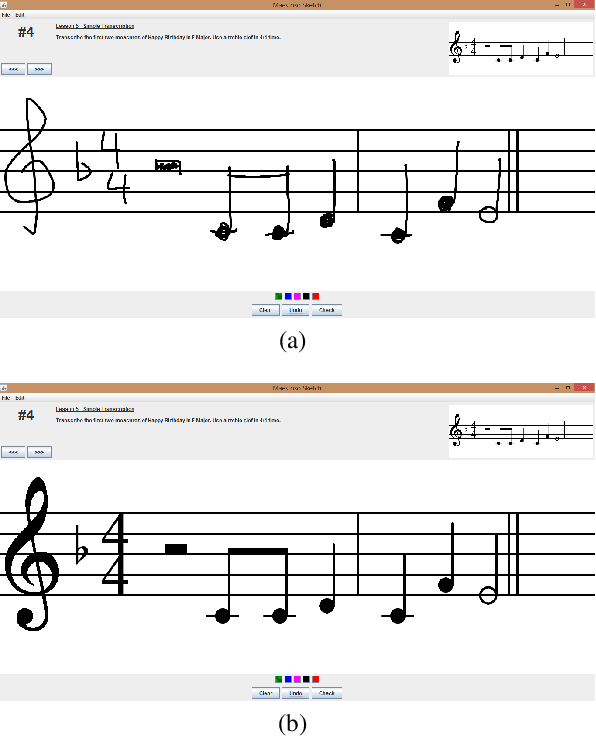
\includegraphics{images/maestoso.png}
   \caption{Maestoso Educational
   Sketching Tool for Learning Music Theory}
   \label{fig:taele2015maestoso}
\end{marginfigure}

The work of Taele et al. \cite{taele2015maestoso} \ref{fig:taele2015maestoso} describes the practical and cognitive benefits of learning music theory for both musicians and non-musicians. The paper proposes an intelligent educational tool to help students learn music theory. The tool, called Maestoso, utilizes sketch-based interaction and machine-learning techniques to provide personalized feedback to the user.
The paper first introduces the importance of music education and the challenges students face when learning music theory, such as the abstract nature of music concepts and the difficulty of translating musical ideas into notation.
Maestoso is a sketching interface that allows users to draw musical notes, chords, and melodies using a stylus or finger. The program uses machine learning algorithms to recognize the user's sketches and provide feedback on their accuracy and completeness.

\begin{marginfigure}
   \centering
   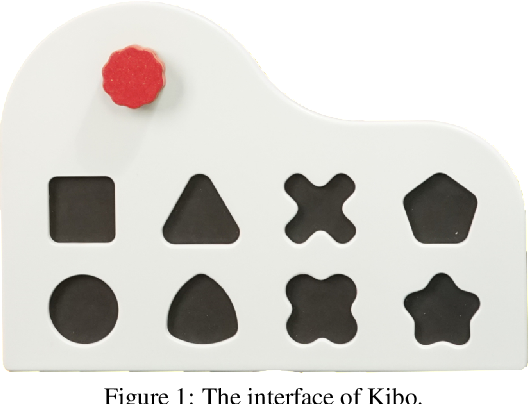
\includegraphics{images/IS_kibo.png}
   \caption{The interface of Kibo}
   \label{fig:amico2020kibo}
\end{marginfigure}

Amico et al. discuss the development of a new type of MIDI controller designed for music education \cite{amico2020kibo}. The device, called Kibo, is a tangible user interface that allows students to interact with music physically and intuitively.
The authors introduce the concept of tangible user interfaces and explain how they can be used to create more immersive and interactive learning experiences.
The device includes a set of modular blocks that the user can rearrange and customize to create different musical experiences.

Implementing such systems is often fully digital and interactive through a screen. Some projects aim to teach children music theory or interact with notes to compose, learn and experiment. Most of these projects are applications that users can download on smartphones or tablets. The relationship with the tangible paper score is gradually lost, and digital interaction replaces it more and more.

One solution is to use conductive ink to keep a tool in paper form without losing its interactive aspect. Conductive inks, paints, and varnishes are liquids containing metal particles, conductive polymers, or graphite. They have the specific ability to conduct electricity.

% TODO AJOUTER LES REFS AUX MARGINFIGURES

\begin{marginfigure}
   \centering
   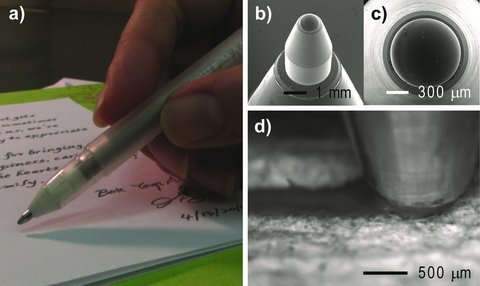
\includegraphics{images/IS_pen-on-paper.jpg}
   \caption{Pen-on-Paper Flexible Electronics. a) Optical image of a rollerball pen loaded with conductive silver ink. b) and c) side and top views of the rollerball pen. d) Optical image of the rollerball pen tip writing a conductive silver track}
   \label{fig:IS_pen-on-paper}
\end{marginfigure}

Inkjet printing allows to pattern of organic semiconductors \cite{kim2008heterogeneous}, metal contacts on organic semiconductors \cite{khan2019soft} \cite{wessely2020sprayable}, and metallic structures that require minimal further processing. Researchers such as Ahn et al. used conductive ink printing to realize metallic connections between functional components of flexible devices.



Another project like that of Russo et al. \cite{russo2011pen} has resulted in an optical image of a flexible paper display containing a LED array \ref{IS_pen-on-paper}. The prototype is a multi-color 25 × 16 LED array connected to the printed silver electrodes by depositing a drop of concentrated silver ink.

\section{General Architecture}

\subsection{Overview}




Our design augments a traditional paper score in many digital music learning applications on screen-based devices. Children already spend a considerable amount of time in front of screens, which can harm their eyes from a young age. Paper is flexible, lightweight, and easily transportable, and incorporating electronic circuits in the paper has shown its attractiveness to children \cite{hershman2018light}. 

\begin{figure}[h]
   \centering
   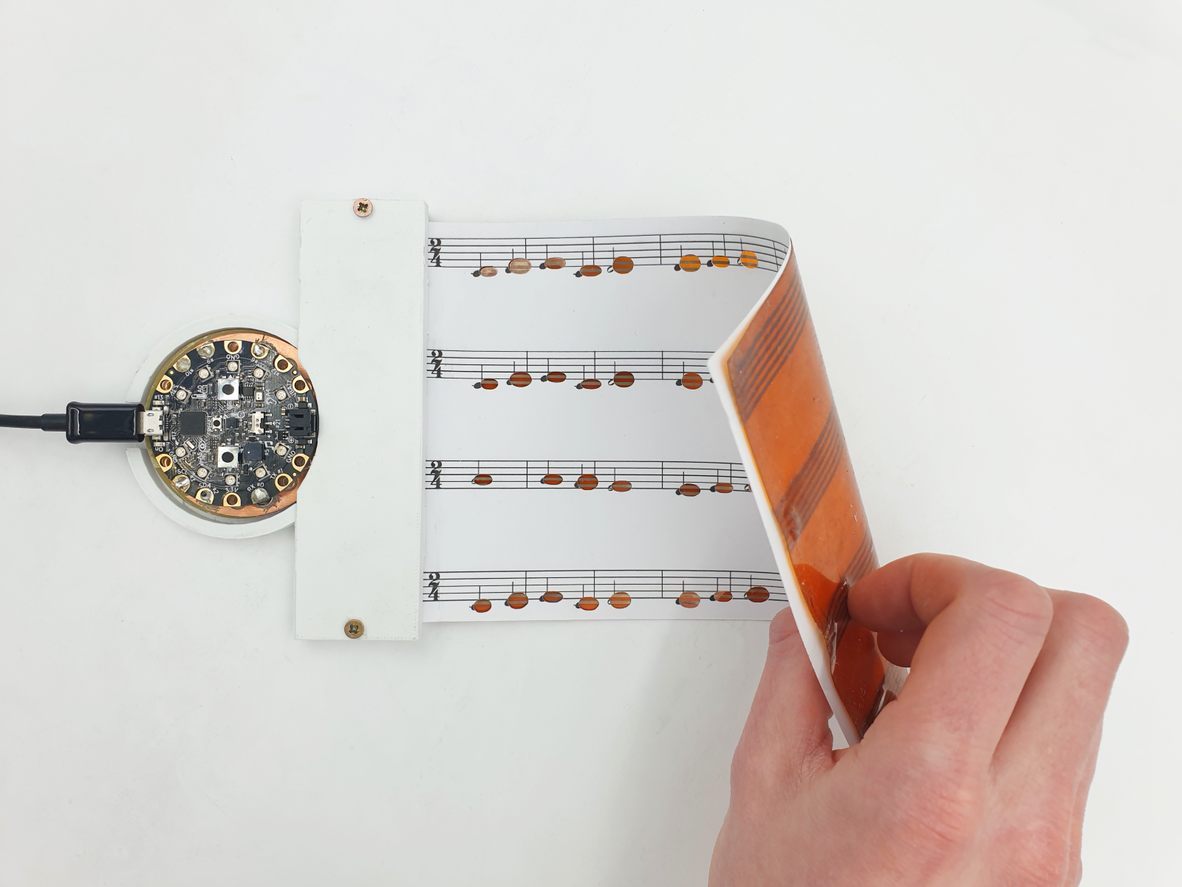
\includegraphics{images/IS_demo.png}
   \caption{Interactive Score Prototype}
   \label{fig:IS_demo}
\end{figure}

The project does not aim to teach a user how to play music. It seeks to link music theory directly with music practice without requiring knowledge.

The user has to supply the electronic part (substrate and PCB), then he places a partition (a cardboard stencil) on top of the substrate (where
the conductive lines are located) \ref{fig:IS_demo}. He can play the music and change it to another one.

\subsection{System Design}

The Interactive score consists of two thin layers. The first layer is the traditional sheet
music, printed on cardstock paper, with holes punched for each note. Under this sheet
is a polyimide substrate with conductive lines printed on it \ref{fig:IS_schema}.

\begin{figure}[h]
   \centering
   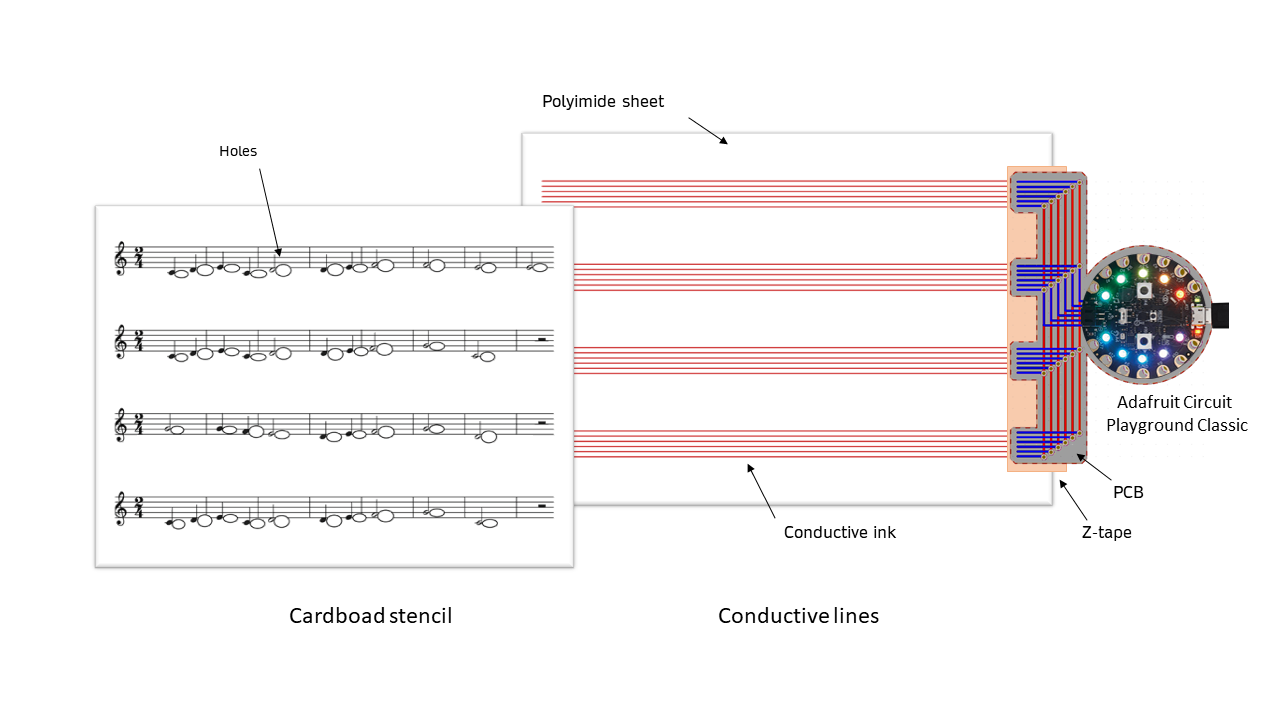
\includegraphics{images/IS_schema.png}
   \caption{Interactive Musical Score architecture.}
   \label{fig:IS_schema}
\end{figure}

The conductive lines are connected to an Adafruit Circuit Playground printed circuit board (PCB) using a double-sided "z-tape".

When the user touches a note on the top layer, the finger makes contact with the conductive lines through the holes in the cardstock.
The signal travels through the ink paths and the z-tape to the PCB, which detects a potential difference using capacitive touch and plays the relevant note. Detecting several simultaneous signals on multiple pins allows playing eleven different notes with only six lines \ref{fig:IS_schema}.

The system is kept in a 3D printed case, maintaining contact between the polyimide, the z tape, and the PCB. The user can easily open and close the case to change the music.



\subsection{Electronic Music Box}

The signal is recovered and used in capacitive touch with an Adafruit Circuit Playground Classic \ref{fig:circuit_playground_classic}. An Arduino program allows for generating a vast number of different notes. The code is retrievable on GitHub \cite{adrien2022capacitive_to_notes}.

\begin{marginfigure}
   \centering
   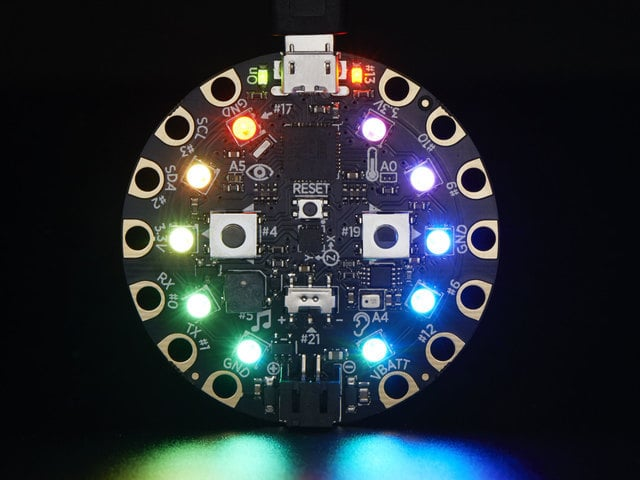
\includegraphics{images/circuit_playground_classic.jpg}
   \caption{Adafruit Circuit Playground Classic}
   \label{fig:circuit_playground_classic}
\end{marginfigure}

About the sound, the Adafruit Circuit Playground embarks a built-in buzzer. The implemented Mini Speaker is the SQMS5002S4036A. This device is a miniature magnetic speaker not adapted for playing detailed audio but for beeping, buzzing, and simple bleepy tunes. It is also possible to change the tone by changing the name of a variable in the code on the microcontroller.

The Adafruit circuit playground has ten mini NeoPixels of all colors, which can be animated with light when a user plays a note. The controller includes motion, temperature, light, sound sensors, a switch, and a mini speaker. This device is ideally suited for use on the score and integrates many features.

\subsection{Paper Score Manufacturing}

Notes, staves, lines, hyphenation, and cutouts were all placed on the same project for perfect dimensional compatibility between the different elements of the score. It allows the elements to fit together perfectly and export the cutout locations at the correct size relative to the partition's rest.

An inkjet printer draws all cardboard lines, hyphens, notes, and numbers.

A score of "J'ai du bon tabac" (on the left) lies on the substrate. Then, the notes were isolated in another PNG file, selected on Cricut design, and cut directly into the cardboard with Cricut maker 3.

% TODO Justifier les choix techniques

\subsection{Conductive Sheet Manufacturing}

The conductive ink paths are 1mm thick and 5cm long, with a resistance of 0.07 Ohms. A simple inkjet printer equipped to print with silver nanoparticles conductive ink drew the lines directly on the substrate. A hoven sintered the printed patterns at 180°C for 73 minutes. This process allows the quick production of flexible circuits \cite{khan2019soft}.

\begin{figure}[h]
   \centering
   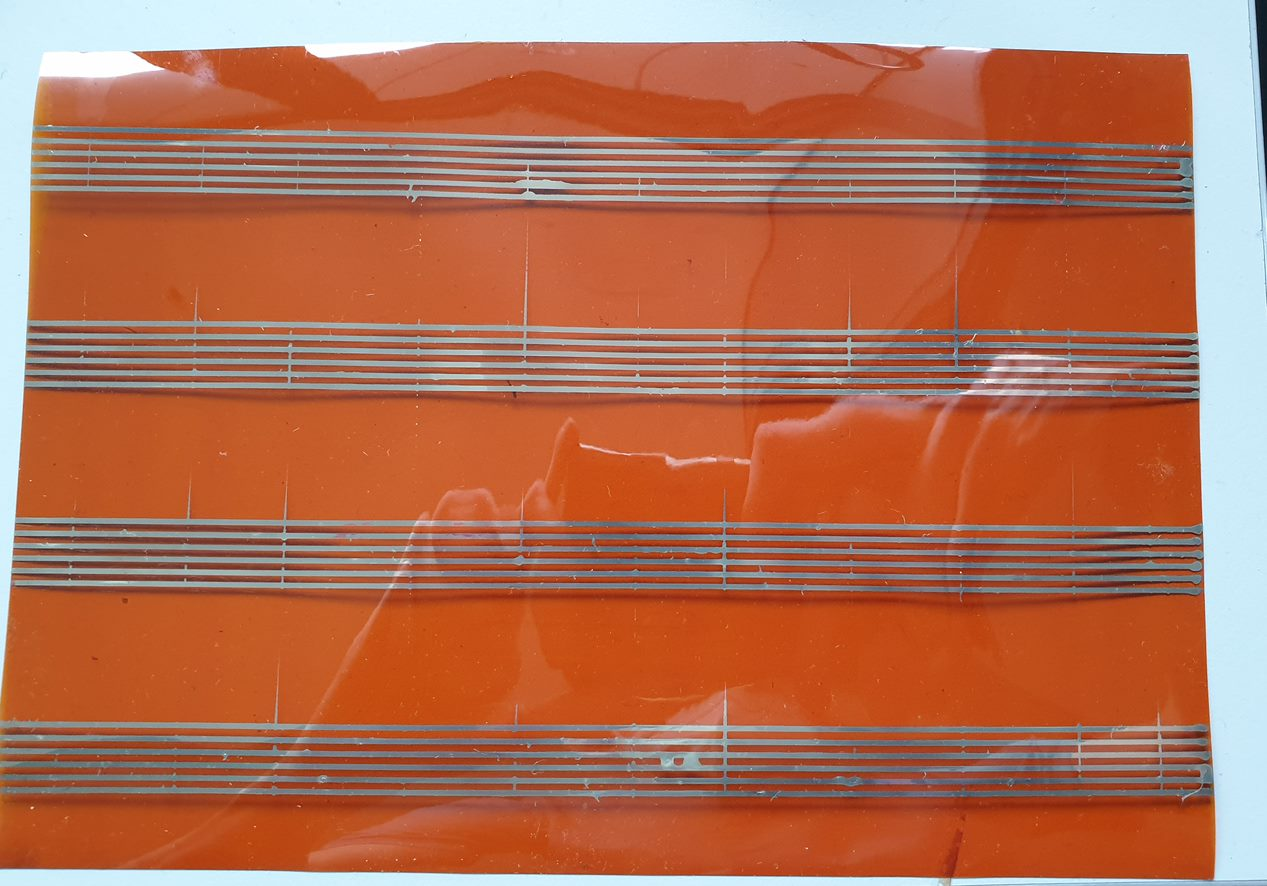
\includegraphics{images/IS_conductive_sheet.jpeg}
   \caption{Interactive Score Conductive Sheet}
   \label{fig:IS_conductive_sheet}
\end{figure}

This prototype comprises four staffs of 6 lines made of conductive ink on a Kapton polyimide sheet substrate. This polymer does not melt at high temperatures and has excellent mechanical strength, and is very dimensionally stable and creep resistant at temperatures above 260°C. The lines are 1mm thick, and at a distance of 15cm in length, it gave a resistance of 0.07 Ohms.

An Epson WF-2010 printer printed the lines on the substrate \cite{adrien2022capacitive_to_notes}.

Conductive ink allows the score to be flexible, like an actual musical score. The use of ink rather than flexible brass strips has the advantage of quickly printing interactive scores on an industrial scale. The material needed is only simple printers and ink and cleaning products for the printers. This process facilitates and accelerates production possibilities.

\subsection{Integration and Usability}

\subsubsection{Ability to change the score}

Its ease of interchangeability and production characterizes the paper score. The user can easily remove the paper sheet from the box and place another to play a different melody. All the electronic parts (substrate, PCB, microcontroller) are independent of the paper score. The sheet music has the exact dimensions of the substrate.
Therefore, placing the two precisely on each other to align the holes with the ink lines is simple.

\subsubsection{Ability to improvise}

The user can improvise by not playing the notes in the same order.
The project allows a great deal of modularity in its use. Just by touching specific notes at certain times, users can experiment with different rhythms and melodies and reconstruct a piece from a few notes.
With a simple score, including an ascending scale, he can try his hand at composition.
It is impossible to create dissonance as the Circuit Playground plays melodies in a fixed tonality set in the code. Unfortunately, this fact also limits the improvisation capacity.


\section{Applications and Evaluation}

\subsection{Set up}

Four users interact with the prototype already prepared for use. They then answer several questions. The project is plugged in and set up as a base for further use. Therefore, measuring the openness and visualization of music theory given by the project to the user is interesting. The questions concern understanding use, practicality, interest, innovation, attractiveness, and playfulness.

\subsection{Results}

The users did not encounter any particular problems during the test. The prototype worked well. The testers gave interesting feedback. The majority of the comments were positive, as the project considered most of their comments since a previous test.

The users proposed many ideas to make the project evolve. They advised adding indications, potentially with LEDs, to indicate actions to be carried out. One idea was to create a binder with different stencils inside. They would have appreciated a correction of the electronics, which would warn them if they made a mistake. The testers liked that the person playing has to press the right notes, unlike some music toys that automatically correct the sound to play the right notes wherever the user presses. The users were also very interested in the fact that the project is portable. They would have liked to be able to take it with them to play music everywhere.

\section{Discussion}

\subsection{Attractivity}

The project is attractive for children as a tangible object.
Its gamified aspect makes it close to a toy. This aspect contributes to its attractiveness, especially to young children. Its musical property favors the user's creativity in addition to being portable, tactile, fun, and easy to use.

\subsection{Musical Imagery learning}

An essential aspect of musical practice is the ability of the musician to decipher a score. When this one practices with visual support, his brain must take the exercise to connect the note, which he links visually with the position of his fingers on the instrument. The transcription of the note read is an intermediate the brain uses, deducing a position and calculating an interval from it. The ability to translate a visual note into a sound is a reflex to be trained and very relevant in the practice of music. The basics of this ability must be acquired very quickly when learning the basics of music.

\subsection{Mobilising multiple intelligences}

This kind of device has a genuine interest in terms of learning. The user practices bodily intelligence with touch, visual intelligence since he has a support in front of him, and musical-rhythmic intelligence.

\section{Conclusion}

In conclusion, the interactive score project has a bright future, as it implements a very recent technology to popularize it. This process could be industrialized and even replicable for individuals with some improvements and optimizations. In the future, our goal is to make the score more accessible. Features such as flexibility and a simple "plug and play" aspect make it attractive even to children.

\subsection{Limitations}

The project has some limitations being a prototype. The device is limited in terms of the number of playable notes. The conductive sheet has six lines of conductive ink, which allows for playing 13 different notes between C5 and F6. It is not possible to generate alterations while playing. This fact means that if the playground circuit is set in a specific key, it is impossible to play a note with an alteration not present in the score's framework. The key must also be changed manually at each score change (paper sheet).

The major problem of the prototype is in its transmission of electrical signals.
The most crucial problem of the project is its sensitivity to the electric field due to the use of capacitive touch. Near electric fields, the microcontroller can detect false contacts. The device must also be connected to a power outlet so that the potential difference calculated between the user's finger and the ground is remarkable. Otherwise, the playground circuit may not detect the touch of a line or start playing by itself because of the detection of surrounding electric fields. A user should therefore keep the device at a distance from electronic devices and metal surfaces.

Z-tape transmits the signal from the conductive sheet to the PCB (inside the box). This conductive tape can be damaged and cause false contacts after many uses and transport. The tape can not transmit the current to the lines, and some notes stop working.

Another problem is the conductive ink which can crumble, preventing the current from crossing certain lines. The ink traces are indeed quite fragile and easily damaged. The ink is only dried on the substrate, so its adhesion can weaken. As the user has to run his finger over the ink, he can also remove thin layers, thus causing some lines to break.

The prototype also presents a difficulty in overlaying the sheet paper on top of the polyimide sheet to align the notes with the ink lines while keeping a flexible system. The case was designed for this purpose but could be more effective.

The device also needs to be improved in terms of sound quality.
The speaker driver circuitry is an on/off transistor, so the device can only play square waves. The device's loudest frequency is around 4 KHz. The sound generated is shrill, very electronic, and of poor quality. It can thus slow down the desire to practice and does not resemble the sound of an instrument.

\subsection{Future works}

Adding the play of an alteration with three "buttons" usable thanks to the capacitive touch: flat, sharp, and natural, which the user can trigger with the index finger of the left hand, is an idea to answer the problem of changing the key. These buttons will allow the user to discover the notion of these three tools and their meaning. They would be an interesting tool that would add an improvisation capacity to the system.

A "musical tutorial" should be added so the user can listen to the score's music before playing it. The tutorial would allow the user to assimilate the musical rhythm (the time between playing each note) with the physical rhythm (the time between pressing notes).

The electronic PCB/microcontroller part should also be redesigned to no longer integrate an Adafruit Circuit Playground but a much smaller, handmade circuit. It would be possible to improve the speaker's quality and connect the device to Bluetooth or Wi-Fi to play music at a distance.
The next steps are also about looking for partnerships in children's education to research experimentations on the impact of this interactive score on music assimilation. Several parameters would be evaluated, such as concentration level, playing time, and knowledge retention. It is necessary to consider different strategies to transcript musical-rhythmic on this interactive score.

    \chapter{Sign Language Learning Game in AR}

\section{Introduction}

Sign Language is considered the main communication tool for deaf or hard of hearing people. It is a visual language that uses movements to provide people communication with the world. 

This sign language is too little used because it requires a significant investment to learn it and most people do not use it directly in their lives. SL is not understood by everyone, forming a communication gap between the mute and the able people. According to the World Health Organization (WHO) report, the number of people affected by hearing disability in 2020 was 466 million whose 34 million are children \cite{el2020sign}. Over 900 million people will have this disability by 2050.

In France in 2020, there were approximately 4 and 5 million deaf or hard of hearing people who have difficulties or are simply unable to communicate through speech. Concerning the deaf speakers of French Sign Language (LSF), the figures are uncertain: they oscillate between 80,000 and 120,000, depending on the sources.

In this work, we introduce a short video game to teach sign language. The application is intended to work on the DVIC Interactive Mirror but is fully functional on a simple PC.

This report deals with the implementation of an AI for sign language recognition (SLR) using the mediapipe framework in order to extract the user’s coordinates and to analyze them through a model in pytorch. The model is then implemented in a game engine to create a visual novel video game. The game is then adapted to an augmented mirror to allow the user to play it in augmented reality. The game stimulates the motivation of the player in order to favorise his learning.

\subsection{GOSAI for Augmented Mirroir}

GOSAI is a new framework to help the development of augmented interfaces on the computer with a display. This framework targets all developers, from beginners to experts. GOSAI offers
basic and often used augmented reality functionalities.

Its structure allows for components to be reused between
projects, thus building a general catalog of tools and
solutions that develops over time.

In addition, the framework uses mainstream programming languages to allow a wide range of developers to
use it. The framework is written in Python and Javascript.
Python is used for the framework’s core components,
while Javascript is used for display.

JavaScript is a flexible programming language. It is one of the core
technologies of web development, and everyone can use it on both the
front-end and the back-end.
It is a versatile and robust language for video game. The developers can use JavaScript to make games using a variety of platforms and tools. They can use both 2d and 3d libraries in combination with JavaScript to create fully-fledged games in the browser or external game engine platforms \cite{javascriptgaming}.

The following projects presented in this thesis are implemented on an augmented mirror running on the GOSAI software system.

The augmented mirror is a platform that provides extensive interaction between the real and the virtual world. The objective is to create a platform that can provide not only recreational use but also medical and educational use.

A one-way mirror is placed against a screen. The mirror reflects perfectly where the screen is black and can display  information when the pixels are emitting light. A camera is placed at the top of the mirror, facing slightly down.  A laptop is placed at the back of the screen.

The mirror can scan the room and detect and position objects the user interacts with. The augmented mirror uses the Intel D435 camera to estimate the position of a user in front of the mirror with Mediapipe. Thus, it can add a new dimension of interaction exploiting kinesthesia. This dimension is an advantage over traditional interfaces using touch or a mouse. 

This interface is ideal for the development of applications requiring movement. This is why it is relevant for the implementation of AI-assisted sign language learning modules.

\section{Related work}

\subsection{Sign Language Recognition}

A wide range of domains use SLR for different purposes. It can be found in robotics, human services, games, virtual reality applications, direct or remote communication or HCI projects \cite{adeyanju2021machine} \ref{fig:Polhemus}.

\begin{marginfigure}
    \centering
    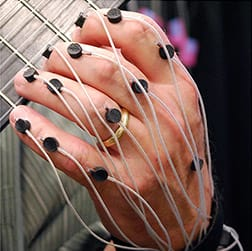
\includegraphics{AdrLfv_master_thesis/images/polhemus_tracker.jpg}
    \caption{Polhemus}
    \label{fig:Polhemus}
\end{marginfigure}

Many early SLR systems used data gloves and accelerometers to acquire specifics of the hands. The devices mesure x,y,z, orientation, velocity directly using a sensor such as the Polhemus tracker \cite{413199} \cite{5738842} or DataGlove \cite{Kadous1970} \cite{Metaxas1970} including accelerometers, gyroscopes, and electromyography sensors  \ref{fig:data_gloves}. Those techniques did not allow full natural movement and constricted the mobility of the signer, altering the signs performed and being restrictive because of the need of supplementary material.

\begin{marginfigure}
    \centering
    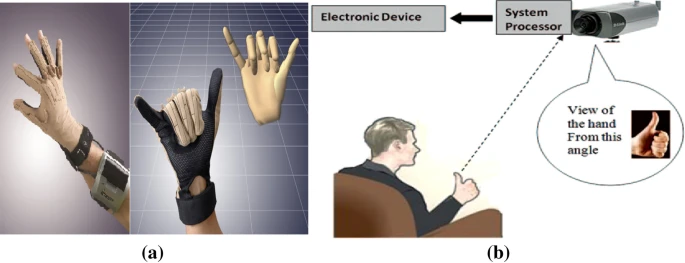
\includegraphics{AdrLfv_master_thesis/images/data_gloves.jpg}
    \caption{Human–computer interaction using: a CyberGlove-II \cite{cyberglovesystems}, b vision-based system}
    \label{fig:data_gloves}
\end{marginfigure}

Most techniques based on data gloves convert the position of fingers and hands according to their angles into electrical signals to obtain the desired sign. 

In 2010, the ImageNet files appeared \cite{li2010crowdsourcing}. They provided a basis for the CNNs and deep learning models used today. This was the beginning of computer vision. In 2012, AlexNet appeared and dramatically reduced the error rate for image recognition \cite{alom2018history}. After the appearance of these models, the use of data gloves is gradually abandoned to focus on the implementation of modules using computer vision.

Computer vision based techniques use pose estimation on the face, body, hands and fingers to detect their position. This method uses images or videos of the signs through the use of a camera and calculations on the images assisted by artificial intelligence \cite{adeyanju2021machine}. 

The identification of signs must take into account many different parameters. Facial expressions and body posture are key in determining the meaning of sentences, e.g. eyebrow position can determine the question type. Some signs are distinguishable only by lip shape, as they share a common manual sign \cite{cooper2011sign}. 


\begin{marginfigure}
    \centering
    
    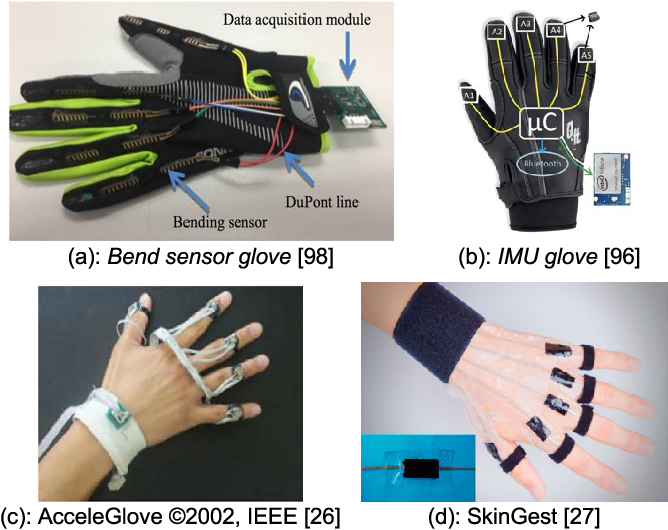
\includegraphics{AdrLfv_master_thesis/images/8-Figure2-1.png}
    \caption{Various custom gloves constructed by researchers in the sign language recognition field.}
    \label{fig:8-Figure2-1}
\end{marginfigure}

The speed of the sign realization can change the notion of speed induced by the performed sign. A sign can also depend on its position on the body. All limbs must therefore be taken into account during the analysis. These challenges include sensor placement, data collection and preprocessing, and model training and evaluation \cite{9178440} \ref{fig:8-Figure2-1}.

Sign language recognition systems based on computer vision and wearable sensors have been proposed by several researchers \cite{ionescu2005dynamic} \cite{yu2010vision} \cite{li2015feature} \cite{sonkusare2015review} \cite{bobic2016hand} \cite{islam2017real} \cite{islam2017real} \cite{saha2018machine}, \cite{rastgoo2021hand} \cite{xu2021application}. 

\begin{marginfigure}
    \centering
    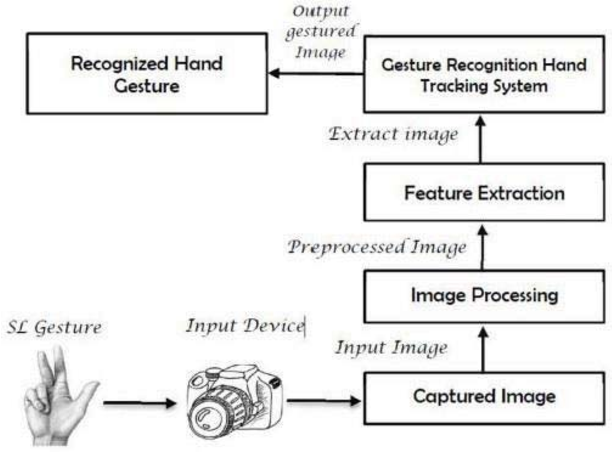
\includegraphics{AdrLfv_master_thesis/AdrLfv-main.tex/images/2-Figure2-1.png}
    \caption{Typical Vision Based Sign Language Recognition architecture.}
    \label{fig:2-Figure2-1}
\end{marginfigure}

Most recent SLR techniques use various image or vision based SLR systems comprising feature extraction and classification \cite{nimisha2020brief} \ref{fig:2-Figure2-1}. 

Many projects using computer vision assisted SLR exist \cite{admasu2010ethiopian} \cite{deriche2019intelligent} \cite{ahram2021advances} \cite{song2021intelligent} \cite{lee2021american} \cite{lee2021comparative} \cite{gao2021rnn}. 

A large part of these projects use a Convolutional Neural Network (CNN) model for predicting American Sign Language alphabet \cite{bin2019study}. Previously, different classifiers like support vector machine \cite{savur2015real}, random forest, multilayer perceptron, transfer learning, fine tuning \cite{saleh2020arabic} etc. have been introduced for sign language recognition on simple images. Recently, shallow CNN and Capsule Networks have obtained better results \cite{hasan2020classification}. 

Skeleton coordinate-based action recognition with coordinates has recently been attracting more and more attention to compute sign language videos because of its invariance to subject or background, whereas skeleton coordinate-based SLR only takes the data that is important for its learning. 

The most commonly used pose estimation frameworks that extract coordinates from a person using pose estimation are for example OpenPose \cite{cao2017realtime} \ref{1-Figure1-1}, MoveNet \cite{movenet}, PoseNet \cite{kendall2015posenet} and MediaPipe \cite{lugaresi2019mediapipe}.

\begin{marginfigure}
    \centering
    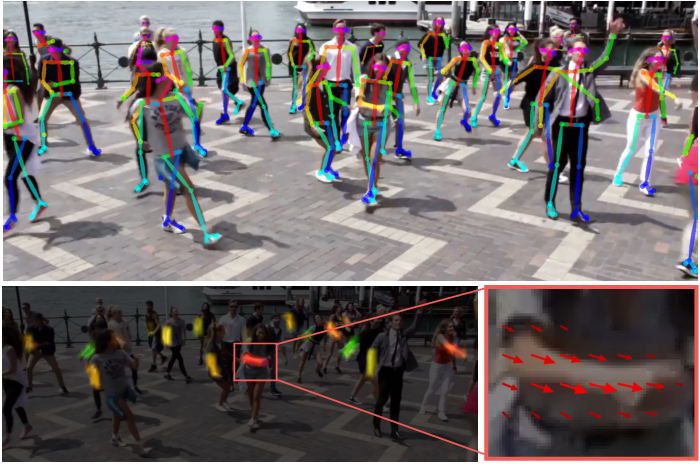
\includegraphics{AdrLfv_master_thesis/AdrLfv-main.tex/images/1-Figure1-1.png}
    \caption{Top: Multi-person pose estimation. Body parts belonging to the same person are linked, including foot keypoints (big toes, small toes, and heels). Bottom left: Part Affinity Fields (PAFs) corresponding to the limb connecting right elbow and wrist. The color encodes orientation. Bottom right: A 2D vector in each pixel of every PAF encodes the position and orientation of the limbs.}
    \label{fig:1-Figure1-1}
\end{marginfigure}

The recovered coordinates (extracted with computer vision or thanks to data gloves) are then processed with training methods. Various machine learning algorithms are then used for sign language recognition, including neural networks, support vector machines, and hidden Markov models \cite{9178440}.

Adeyanju et al. provides a comprehensive review of the state-of-the-art techniques used in sign language recognition using machine learning \cite{almeida2014feature} \ref{S0957417414003042}. The paper highlights the significance of sign language recognition and its potential to revolutionize the way communication is done between the deaf community and the hearing community. The authors then review the different machine learning techniques used for sign language recognition, such as Hidden Markov Models (HMMs), Support Vector Machines (SVMs), and Deep Neural Networks (DNNs).
The authors also highlight the importance of datasets in sign language recognition and review some of the commonly used datasets for sign language recognition. They emphasize the need for large, diverse datasets to train machine learning models effectively.

\begin{marginfigure}
    \centering
    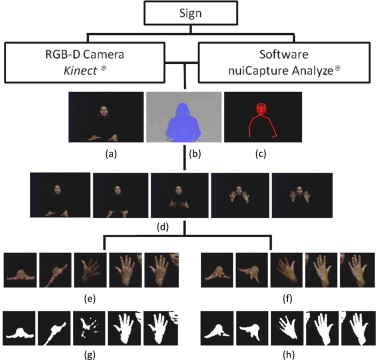
\includegraphics{AdrLfv_master_thesis/AdrLfv-main.tex/images/S0957417414003042.jpg}
    \caption{Feature extraction in Brazilian Sign Language Recognition based on phonological structure and using RGB-D sensors}
    \label{fig:S0957417414003042}
\end{marginfigure}

However, sign language is far more than just a collection of well specified gestures.

%TODO ajouter le concours de google

\subsection{Sign Language Learning Video Games}

The video game is a dynamic audiovisual entertainment platform, accessible and stimulating the imagination of players. There is a possibility of using them to strengthen skills and abilities within society. This is how video games are becoming a playful phenomenon, important in children's and youth culture.
Video games enhance the function of the attentional system, stimulate visual attention, reduce reaction time, improve the ability to discriminate shape and color, plus efficiency when following multiple object \cite{green2006enumeration}.

They are a good didactic way to promote interest and motivation by linking playfulness and pedagogical functions \cite{tejeiro2009efectos} .

The augmentation of interfaces thanks to technology causes a better attractiveness of the learning method and thus an increase of the time voluntarily dedicated to self-learning and of the motivation to concentrate on the method \cite{baker1994}.

Very few games use sign language as a basic element in the gameplay. We can cite Moss \cite{moss2018} \ref{moss-1200-80}, a video game on PlayStation VR in which the hero communicates with the player with ASL. 

\begin{marginfigure}
    \centering
    
\includegraphics{AdrLfv_master_thesis/AdrLfv-main.tex/images/moss-1200-80.jpg}
    \caption{Moss hero communicating with the player through american sign language}
    \label{fig:moss-1200-80}
\end{marginfigure}

Zahoor Zafrulla et al. present Copycat, a game designed to improve the American Sign Language (ASL) skills of deaf children \cite{zafrulla2011copycat}. The game was developed by a team of researchers from the University of California in collaboration with members of the deaf community.
The game, called CopyCat, is a digital game that uses machine learning to provide feedback to the players. The game consists of a series of mini-games that focus on different aspects of ASL, such as finger spelling, vocabulary, and grammar \ref{aslgamecopycat}. In each mini-game, the player is presented with a video clip of a person signing a word or phrase in ASL. The player is then asked to copy the sign or phrase using their own signing.

\begin{marginfigure}
    \centering
    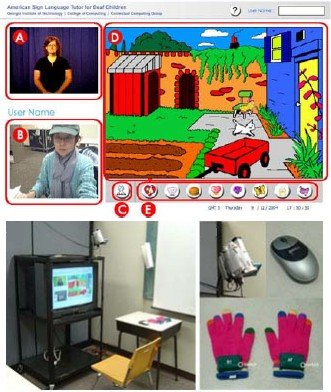
\includegraphics{AdrLfv_master_thesis/AdrLfv-main.tex/images/aslgamecopycat.jpeg}
    \caption{Screenshot of ASL Game Interface and the input devices for user  }
    \label{fig:aslgamecopycat}
\end{marginfigure}

CopyCat uses machine learning to analyze the player's signing and provide feedback on their performance. The game is designed to be adaptive, meaning that it adjusts the difficulty level based on the player's skill level. The game also tracks the player's progress and provides feedback on areas where they need improvement.
CopyCat developpers then enhanced their SLR system with the Kinect depth-mapping camera which uses colored gloves and embedded accelerometers to track children's hand movements \cite{zafrulla2011american}.

Bouzid et al. explore the use of a learning game for SignWriting, a system for writing sign languages, to enhance sign language learning for students \cite{bouzid2016using}. The game is designed to be played on a computer or tablet and includes a variety of activities such as matching signs to their written symbols and translating written symbols into signs.

Lesmes et al. discusses the development of educational video games for deaf children in order to facilitate their inclusion in mainstream educational settings \cite{lesmes2022design}. The paper outlines the design and development process of educational video games, including the use of a participatory design approach that involved deaf children and educators throughout the design process. The games were designed to incorporate sign language, visual cues, and other features that would make them accessible to deaf children.

Many applications on smartphones aim at learning sign language. Some target children by displaying animals demonstrated in 3D (SignEveil).
Most of these applications are in a quiz with a lesson part and a questionnaire part. It is not possible to interact by making the signs yourself.
JavaScript is used extensively in games that do not require many resources. A 2D interactive game displays only a few details and elements.

JavaScript is a language adapted for such a creation. Frameworks like Phaser JS library or simply P5 are suitable for coding a small game. p5.js is a JavaScript library for creative coding, focusing on making coding accessible and inclusive for artists, designers, educators, beginners, and anyone else. It can display graphics and process many different elements.

% Parler de pocket sign

\subsection{Visual Novel Engines}

P5VN is an open-source Interactive Design and Media Major at NYU Tandon School of Engineering student project, allowing to create a visual novel using P5.js. It allows to display dialogues, sprites, as well as backgrounds and use menus by clicking. The game scenario is easily editable through a script, which is then parsed by the engine. The original aim of the project was to implement a prototype engine based in p5.js with a custom scripting language.  

Other visual novel engine, Tuesday JS \cite{TuesdayJS} or Monogatari \cite{monogatari} are simple web-based visual novel editor that can be used in a web browser. They are written in JavaScript allowing the use of vector graphics svg, gif animations and css styles.

Tuesay.js is an easy to use visual novel editor. Free and open source, it runs on any web browser. It is written in JavaScript, does not use third-party libraries and therefore does not require additional software installation. It uses a drag-and-drop interface for editing scenes and creating interfaces. The script is displayed as a flowchart with all the elements and branches of the plot. This makes it easy to navigate and helps you create stories with many plot options.

Monogatari.io is similar to Tuesday.js. The platform support different medias (images, videos, music), multiple languages. It is highly customizable, open source and multi-platform. 

\subsection{Animated 3D Avatar}

For the creation of an animated avatar, most systems implement the display of an animated model from an animation software (Blender, 3DS Max, Maya, Unity, Houdini...). The animations are worked directly in the software and then imported into a program for display in a game. 
Some projects allow the animation of a 3D model directly from the motion capture. In the project "Real-time Avatar Animation from a Single Image" \cite{saragih2011real} Saragih et Al. realize the modeling of 3D models from a simple photograph \cite{saragih2011real}. 

A tool such as Unity or Maya can make its animation from MediaPipe coordinates. A tool that gives nice rendering for 2D animation is Pose Animator. A demonstration works with FaceMesh and PoseNet (from MediaPipe) online \cite{pose\_animator}. Unfortunately, this one does not understand finger movements. Adapting this system to MediaPipe by adding finger movements can give a free 2D avatar. 

Another way is to adapt the coordinates in real-time to animate a character on Blender using Daz Studio as Nguyen et Al. \cite{nguyen2021automatic}.
Many other demos of characters built with MediaPipe exist. Most use MediaPipe and TensorFlow.js (namely FaceMesh, BlazePose and HandPose) \cite{blazepose}.

Another project allows moving a 3D model with Three.js (React Three Fiber) and Tensorflow’s Pose Estimation model (PoseNet). The model uses Tensorflow and PoseNet to detect the key points of the joints in each frame and then send those points over to the Model file. The project uses an Adobe Mixamo 3D model in FBX format and Blender to import the FBX format and export a GLB format \cite{posenet}.

A last interesting example is that of Kalidokit \cite{kalidokit}. Kalidokit is a tool that uses Mediapipe/Tensorflow.js models for tracking face, eyes, pose, and hand movements. It is compatible with various models such as Facemesh, Blazepose, Handpose, and Holistic. The tool calculates simple euler rotations and blendshape face values based on the predicted 3D landmarks.

Kalidokit is the core component for Vtuber web apps, such as Kalidoface and Kalidoface 3D. Its purpose is to rig 3D VRM models and Live2D avatars. The project is a JS library intended for developers using Mediapipe pretrained models and not a complete app on its own. The library still has to be adapted to run on different platforms. The project is based on Three.js, a powerful library for creating three-dimensional models and games. 
With just a few lines of JavaScript, it allows the creation of simple 3D patterns to photorealistic, real-time scenes. The library can create complex 3D geometrics, and animate and move objects.

Three.js enables the application of textures and materials. It also provides various light sources to illuminate scenes, advanced postprocessing effects, custom shaders, load objects from 3D modeling software... It is easy to use, intuitive, and a well-documented library.

\section{Gameplay}

The sign language game is an augmented reality game, a visual novel on the augmented mirror. We follow a character during a short adventure in which the user can take choices by making American Sign Language signs in front of the mirror. He can answer to the characters, interact with objects, choose actions and choose a path. 
Sometimes the player sees the tutorial of one, two, or three signs at the same time. The user must then make the sign of the choice he takes. For example he can choose to turn right or left by making the appropriate sign. 
3D avatars are the models for all the characters. Their limbs (including fingers) are animated. Only the character Aria (the hero's friend) is performing the sign tutorials.
The signs made are detected by the camera and guessed by an AI working in back end. Dialogue lines appear during the adventure to guide and discuss with the player. The user must make the "ok" sign with his hand to scroll the text.


\section{General Architecture}

\subsection{Visual Novel Engine}

\subsubsection{Engine implementation}

The best solution to make such a game was the implementation of a visual novel engine on the mirror from which to develop everything else in the game. P5VN engine is precisely  basically adaptable for the mirror because the engine is basically working with p5.js.

Previouly, p5VN was able to load and display background, sprites of characters, some text interactive with the mouse click, menus with multiple buttons for the user to take choices.
The engine was running synchronously in a single thread.
After an important adaption. The module is now running asynchronously to be compatible with gosai. 
The engine now loads and plays video animations automaticaly at launch, the user can now interact and select menus thanks to sign language and added many other features.

\subsubsection{Menu}

In a visual novel, the player does not interact directly with the keyboard but must click on menu buttons to make choices. As the user interacts with the mirror only by the estimated pose, the menu system had to be adapted to both enable debugging by clicking and making choices with movements.

Each time a menu appears, it takes the form of three words aligned and distributed horizontally on the screen. An avatar of Aria appears behind each word to demonstrate the sign related to this word. The location of the words and the 3D tutorials are spread over the width of the screen according to the number of buttons in the displayed menu. 

Aria's avatar animation plays in a loop until the player makes a sign detected by the SLR module and included in the menu. The path taken by the game is then directed towards the continuity of the chosen branch.

\subsubsection{Script}

The game script is contained in a script.txt file in the application components. It contains a set of commands starting with the \$ symbol telling the game to do a particular action. These commands can be :
\$tag which indicates a specific point in the script
\$jump to jump to a tag
\$defineC to define a character (name, sprite address, text color)
\$defineImg to define an image
\$bg to display a background
\$show to display a character
\$addAnimation to play an animation to a character
\$setSprite to display the sprite of a character
\$menu to create a new menu
\$hide to hide a character
\$setvar to set a variable to a value
\$if to manage if then else commands

All the loading of sprites, animations, their playback, display is now managed automatically at startup in asynchronous instead of being set manually in the script or in the code as before. The engine running in synchronous mode at the beginning, a sprite could not be called before being loaded. The game starts on a loading time at startup corresponding to the loading of sprites and animation videos in the memory of gosai. This allows each animation to be played instantly when each one is called.

\subsection{Animations}

The most efficient way to create accurate custom 3D animations for the animated sign language tutorials was to implement a module allowing to control an avatar in 3D through pose estimation and then record the movements produced or a video of the animation.

An application to control an avatar remotely thanks to the estimation pose has been developed on the augmented mirror. The avatar is able to track and copy accurately the position of the user's limbs. The created application is now in free demonstration on the mirror. It also allowed to create all the 3D character animations on the sign language learning game.

\subsubsection{Esla}

The Educative Sign Language Avatar (ESLA) is a 3-dimensional avatar controllable in a gosai application following the estimated MediaPipe pose. Its movements copy live those of the user in front of the mirror \cite{esla}. It was the first version of the interactive avatar on the augmented mirror.

An animated 3D character appears on top of the scenery at the launch of the application. Its animation is made possible by playing features using MediaPipe and OpenCV. The program can retrieve the coordinates of a user’s position in real time. These coordinates are processed, and the avatar copies the movements Animation Retargeting, a video game animation technique using motion capture.

The programs retrieves the links between each point of the pose provided by MediaPipe and Three.js calculates and display the 3D part. 

Three.js entirely manage the loading of the character, its display, its animation, the rendering, the light and the camera .

Three.js uses a pivot system with matrix4 and quaternions. However, some functions to transfer rotations from one base to
another are missing (even though they are very much in demand by the community). Therefore, the entire limb rotation system was implemented by hand.
MediaPipe first retrieves the (real) coordinates of the user. These coordinates are converted into the world base (x-axis to the right, y-axis to the top, z-axis to the camera) of the three.js scene with transformations. The program retrieves the coordinates of the top of the spine, the shoulder, and the elbow. It creates two vectors spine/shoulder and shoulder/elbow. The coordinates of these two vectors are then read from the base of the parent of the bone to be rotated (here the left shoulder). An algorithm then calculates a quaternion containing the rotation data from the first vector to the second.

This quaternion is then applied to the limb, which takes in its local base the same rotation as the user’s arm with his shoulder.
This allows you to make precise rotation transfers from one base to another and thus animate all parts of the avatar.

Unfortunately, the project lacks a lot of precision in the movements, especially at the level of the fingers, which is very inconvenient for the creation of accurate tutorials in sign language. Another more efficient solution for the creation of 3D animations with the estimated pose had to be implemented.

\subsubsection{Kalidokit module implementation}

The most important part of making the 3D animations the management of the avatar from Mediapipe, it is enabled by the Kalidokit solver. This JS library allowing the animation of arms, hands, fingers, face, mouth, eyelids, pupil of VRM models (Virtual Reality Model). The VRM is formulated on the basis of the standard 3D format glTF2.0 to manage humanoid models. It aims to be particularly expressive. This type of model has a large number of articulations, can blink and animate its mouth. It is very often used in the world of VR games (VR chat for example), or by Vtubers (entertainment broadcasters who use a virtual avatar).  

The models used are downloaded from the site Vroid Hub cite\cite{vroid}. They must respect specific conditions of use: use by a third party, downloadable, use as an avatar, commercial use by a company. The avatar must also be sober. The one that has been selected to be implemented in the demo application allowing to control the avatar in augmented reality on the mirror is called "papa\_de\_him\_chan". 

The model is easily changeable locally in the application created to allow the user to manipulate different characters. It is with this application that will be created the animations of tutorials of sign language for the learning game on the mirror.

Such an application therefore allows to record qualitative signs and poses for the characters and tutorials of the game.

The models used for the characters of Aria, the grandmother and the salesman were recovered on Vroid Hub and are free to use. The VRM models are mainly adapted for Vtubers, that's why the characters can look very childish and like Japanese anime characters.

\section{Sign Language AI}

\subsection{Overview}

Sign language involves the usage of the upper part of the body, such as hand gestures, facial expression, lip-reading, head nodding and body postures to disseminate information \cite{adeyanju2021machine}.

The final goal of this work is to implement an SLR AI inside the sign language learning game. This AI allows the recognition of choices in the game thanks to the esimation of the user's pose but also the control of the game using commands linked to signs.

Many models with sign language recognition already exist. The work done here proposes a model, as well as an easy system of creation, dataset management, training and visualization of the data.

\subsection{Integration in Gosai}

The project of creating the SLR AI is apart from gosai \cite{slr\_mirror}. Only the weights are integrated in gosai in a module making the comparison between a sign made in front of the camera and the values of the weights recorded locally.

The video game retrieves the coordinates of the user and place them in tensors containing the data of a video of 30 frames.

The model is called by passing the data to it and a table of probabilities concerning each action is retrieved as a result. 

The guessed sign is then transmitted from the slr module through gosai’s redis database to the game engine. When the probability of a detected sign overfits a threshold, the sign is considered as validated by the game engine.

\subsection{Structure}

The project is divided into 6 different local modules and a main file that initializes the parameters and launches the different processes. The processes are an optional phase of dataset creation, a tutorial phase that displays the skeleton for data vizualisation, a preprocess phase that retrieves the data from the dataset and formats them, a data augmentation module, and a weight calculation and exportation in different file types.

\paragraph{Dataset}

If a movement is included in the known actions but is not found in the files, the creation of the dataset of this movement is launched automatically. 

The dataset is created by the user and stored in a folder "MP data" created, and separated in three
folders : train, valid, test containing the actions (name of the
movement). The recorded sequences are automatically separated
between the three folders train (80\% of them), test (10\%) and valid
(10\%). Each sequence is 30 frames each by default, including coordinates, that is to say and now 116 data per frame (that is to say 58 points) after having removed  431 points of the face and just Keeping 4. The 4 kept points are one for the chin, for the forehead, for the wright and left cheek.
It enables signs using the head to be better detected.

The coordinates are retrieved from Mediapipe during the creation of the dataset. The recording is done from the webcam of the device used, an intel real sense or the default pc webcam if the intel is not detected. When implementing on another device such as the interractive mirror, this driver must be modified to match that of the camera used.

At the start of the dataset creation, the user alternates one second of video recording, then two seconds to reposition in a loop for each sign. He has a video feedback on himself to check if he is well positioned in the plan.

\paragraph{The recorded signs visualisation}

The recorded signs visualisation module (data\_vis) retrieves the coordinates of a video by action, stored in the dataset.
It sorts the coordinates of the points of each part of the body,
finds the different links between each point and the posters, frame
by frame. Arrays of all the sorted coordinates for each body
part (Face if activated, Body, Hand) are used, as well as all the links
of the body arrays.

For each point detected in the dataset, the visualization displays the links it has with the points it is linked to in the table. The program also display the action to which the visualization is associated, above the drawn character.

\paragraph{Preprocess}

The preprocess phase retrieves all the data from the dataset and places them in tensors to provide them to the model.
After creating the preprocess instances (according to their type: train, test, valid) we pass them to the dataloader. 

These pass an index to them (concerning a sequence among all the sequences attributed to the type of the preprocess). Their program calculates which action is concerned by the desired sequence and recovers all the coordinates of the frames of this sequence. 
In some papers, it is said that some sign language movements are only possible by giving some indications with lips or facial expressions \cite{cooper2011sign}. Some of the lip coordinates should therefore be kept in the dataset retrieval during the preprocess. For other papers, it is just not necessary to keep these points which take a lot of storage for nothing \cite{dreuw2007speech}.

The preprocess does not use all the coordinates of the face, this allows to have much faster train loops because all these points are not necessary.

\paragraph{Data augmentation}

The data augmentation is called during the pre-processing phase,
just after retrieving the data of the concerned sequence. It is given
the data as a parameter, it reviews the data and will apply a random
horizontal and vertical shift and scale to it. This process artificially
increases the number of positions in which the user can stand.

\paragraph{Model}

The model is composed of a bidirectional LTSM, a linear, a dropout, a batchnorm1d, a relu, and an other Linear. The AI trained on 16 different signs or 1600 sequences. The model reaches an accuracy of 87\% on the test set and 96\% on the training.

Recurrent Neural Networks (RNN) allow to process temporal sequences (language, videos, numerical data). They keep the memory of past data to predict data sequences in the near future. This is why LSTM and Bidirectional layers are used into the model. The LSTM (Long-Short-Term-Memory) are composed of several gates (respectively 3 and 2) which allow to forget or to selectively memorize the information of the previous temporal sequence in a dynamic memory.
LSTMs have an internal memory that is constantly changing dynamically according to the input data sequences.

The training uses the optimizer AdamW, a stochastic gradient descent method that is based on adaptive estimation of first-order and second-order moments with an added method to decay weights \cite{loshchilov2017decoupled}. 

Models are automatically exported in pth format, a common PyTorch convention is to save models. They can also be exported to onnx (Open Neural Network Exchange) \cite{onnx}, an open format designed to represent machine learning models. This extension enables greater interoperability in the AI tool community, allowing a large number of AI frameworks to be more compatible by allowing them to share models. This interoperability allows trained models to be easily deployed in different software platforms like GOSAI.

The onnx models retrieved from the project output are then directly implemented in the SLR module of gosai.

%TODO Ajouter une image des résultats

\subsection{Configuration}

All the processes mentioned above are optional. This management is located in a config.json file in which the user can enable or disable a large number of project features. 

All the options are : "actions" (all the signs recognized by the AI, "adapt\_for\_mirror" (to transform the coordinates specificaly for the augmented mirror),"convert\_files" (to convert the files from pth to onnx), "erase\_dataset" (to erase the dataset before recording a new one, by default the program automaticaly completes the existing dataset), "erase\_runs" (erase the local tensorboard files), "make\_data\_augmentation", "make\_dataset", "make\_train", "make\_tuto"  (visualization of the recorded movements), "nb\_epochs", "nb\_sequences" (total video number the user wants to record for a sign), "sequence\_length" (one video frame number).

The default actions are "nothing", "empty", "ok", "yes", "no", "left", "right", "house", "store", "hello", "goodbye", "television", "leave", "eat", "apple", and "peach". Those are all the signs used inside the SL video game.

The project aims for making it as easy as possible for the user to create weights according to his desired characteristics.

% ajouter schéma du modele
% parler de la visualisation des résultats

\subsection{Visualization of the results}

TensorBoard is a tool providing visualization solutions to machine learning tests. It allows to track and visualize metrics such as loss and correctness. TensorBoard allows displaying the graph of the exported model, displaying histograms of weights, biases or other Tensors, and many other functions.

Just by entering the "make set-up\_tensorboard" function in the terminal (or by doing a "make first\_boot"), the user launches the creation of a local server running on port 6006, retrieving the weights as the model is trained. 

A browser page then opens automatically to access the local server address. On this page the user can study a graph of the training and test phase (percentage of success according to the number of epochs). 

The logs of these results are stored locally, they are accessible and can be easily compared between them. This makes experimentation easier and more intuitive.

\subsection{Limitations}

After many experiments, several biases have appeared that directly affect the AI results. For example, the size of a user differing too much from the person who created the dataset is sometimes problematic, resulting in a strong difference in recognition performance between users with the same or different morphology. 

Since the AI bases its training on the data obtained from Mediapipe, the results of the SLR also depend on its parameters. It was observed that Mediapipe was better at recognizing the limbs of a person with a strong contrast with the background. 

This resulted in a very significant difference of about 15\% in performance on the training and test set. When the dataset was created by a person wearing a black shirt, his white skin was better detected by Mediapipe and better recognized afterwards. 

The same thing happened when using the sign recognition directly, with a t-shirt allowing a better contrast, the recognition was only favored. This also causes the fact that signs made on the belly (being a plain background without detail) are much better recognized than those made on other places with more potential details in the background.

\section{Usage scenario}

The augmented mirror is primarily aimed at families and is designed to be placed in a living room. Its use is very wide and allows to have fun as well as to learn by interacting.
The mirror does not require any additional material, so its use remains very simple.
The learning game of the sign language is directly launched from the menu of the mirror. The user just has to follow the instructions given by Aria to follow the course of the adventure. The game is primarily aimed at young children. Through repetition and distraction, they intuitively learn certain gestures.

\section{User study}

\subsection{Set Up}

As the sign language learning game is intended for young users, this test focuses on a sample of 12 people between 18 and 25 years old.
6 people watch a number of video sign language tutorials on the "pocket sign" application. The signs viewed correspond to those encountered in the game when choosing the path through the house ("ok", "yes", "left", "right", "house", "store", "hello", "goodbye", "television", "leave", "eat") or the path through the store ("ok", "yes", "no", "left", "right", "house", "store", "goodbye", "apple", "peach"). 4 people view the signs of the passage through the house and 2 view the signs of the passage through the store.
When they think they have understood the sign viewed, they skip to the next sign. 

6 other people use the sign language learning game on the mirror. They are told the principle of the game before using it. Two of them go through the house and four of them go through the store.

Both groups are told at the beginning that they will be evaluated on certain signs at the end of the study. 
For both groups, the session is timed from start to finish.

\subsection{Results}

\paragraph{Sign Language Video Game}

In one session, users took an average of 4.44 seconds from game launch to completion. Some users have experienced problems related to poor AI recognition.
Notably for the sign "peach" and the sign "eat" difficult for two users.

One user took 8:25 to complete the game. He had great difficulty in making the "go" sign in the house. This bias is explained by the fact that the dataset was created by a tall person (1,84m) and this user had a much smaller height (1,60m). 

Users were tested after their session on some random signs. Their average score was 2.33 signs learned out of 4. The errors made are related to several elements. The AI sometimes finds a sign far too quickly when the user has not yet placed his hands correctly. The user then has no time to look at the signs and make his choice. Another error is related to the fact that when there are three tutorials at the same time (menus with three choices), the user has more difficulty to concentrate on each one and his memorization of the signs is less efficient.

To correct the problem related to the too high detection speed of the AI, increasing the detection treshold value would be an efficient method.

To conclude, people were asked to note on 10 their opinion about diverse questions. Their average motivation to learn sign language in this particular way (with an augmented mirror and the video game) was 7,91/10.
The average fun in interacting notation was 8,25/10. Their ease of understanding what needs to be done had a notation 7,58/10. The practicality of using this learning method (augmented mirror) had a notation of 8,25/10.The effectivity of using this learning method received a notation of 6,41/10. And the capacity of the AI to guess the correct sign was noted 6,11/10.

The global feedbacks were that the avatar sometimes moves his fingers too much and could not be very precise. The fact that the display is in 2D (on the mirror screen) and not in 3D makes it difficult to understand the signs.
One user was blocked by the fact that the characters look like anime characters and not more realistic ones, which can put off the desire to practice.
Some users forgot the "ok" sign to skip dialogues during the game although the sign was shown twice at the beginning of the game. This prevented them from continuing the practice without external intervention to remind them of the sign. 
One user had learning difficulties due to the avatar's movements being considered unclear. Interacting with a real person, however, allowed him to learn more effectively. The lack of accuracy of the AI was also strongly criticized (rated 6.11/10 by users). This accuracy is almost perfect for the creator of the dataset, but low to other users with a different morphology.

The 3D animated tutorials were generally liked and were considered more attractive than simple video tutorials. The fact that the game was implemented on an augmented mirror was praised because this interface is considered to be mainstream and easy to integrate in a living room.


\paragraph{Videos}

%TODO implémenter la seconde partie de la user study 

\section{Discussions}

The SL Game stimulates the visual, verbal and kinesthetic intelligence. 

The visual intelligence is the ability to create mental images, and to perceive the visible world with precision in its three dimensions. Viewing 3D sign language tutorials and having to "decode" the different movements and positions of the avatars' limbs stimulate the user's visual intelligence. The user needs to perceive, to make a mental projection before re-performing the identified signs.

Verbal intelligence is the ability to read, speak easily and connect mental ideas into words. Having to connect a picture to a word in the project leads to the ability to express oneself fluently and therefore to connect the mental idea of a word into a gesture. 

Kinesthetic intelligence is the ability to use one's body in a fine and elaborate way, to express oneself through movement, to control one's body movements well. This type of intelligence is stimulated through play in this project because the brain must translate the mental image of body positions and movements in space into real positions and movements. 

The stimulation of three different intelligences, added to the motivating gamification aspect, favors information retention. The user can remember a particular gesture by the memory of having seen it and projected it mentally, by the memory of having given it a linguistic meaning, and by the memory of having performed it physically in space.

\section{Conclusion}

\subsection{Playful Learning and ASL}

Playful learning and gamification are learning methods that use playful elements to facilitate the assimilation of knowledge. 

Learning video games are a popular form of these approaches and are often used to teach practical skills such as sign language. The use of augmented reality, pose estimation, and artificial intelligence in the Sign Language Video Game creates an immersive and interactive experience for the learner to practice reproducing signs correctly in real time. This approach promotes learning by providing instant feedback and allowing the learner to practice as many times as they want. 

In addition, the use of cutting-edge technology often generates interest and engagement in the learner, which can help to increase motivation and perseverance in learning sign language.

\subsection{Limitations}

The results of the user studies make it possible to extract a certain number of limitations from the project.

The size difference between the person who created the dataset and a potentially taller or shorter user is problematic. This can be solved by applying a compression of the coordinates to the horizontal and vertical axis randomly in the data augmentation or by registering the dataset by people of different sizes.

The dataset produced and used is small. It contains little noise, little variation, and little mixing. The model is also moderately efficient and could be reworked especially with the use of transformers. The model is also trained on few different signs (15). This means that in the case of an enlargement of the dataset, the accuracy would tend to decrease even more. It is therefore necessary that the model and the dataset be reworked in the future.

Another important limitation is the sometimes difficult clarity of avatars in sign language tutorials. The pivot angles of each of the avatar's bones being limited to avoid glitches and ragdolls, it is sometimes hard to record precise signs especially at the finger level. The user must then imitate and learn a model that is not totally accurate. The avatar can be slightly reworked to widen the achievable angles and thus gain in precision.

\subsection{Future Works}

The current system is good for direct practice but too easy because users can afford to just copy the sign. It would be necessary to add an evaluation dimension with signs that come up in the potential choices without giving the tutorials every time. Thus the user will have to force himself to remember and will have a better learning by repetition.

This work has already been done in another application on the mirror similar to a sign language training. The application consists of successive viewings of sign language tutorial videos, practice, and finally correction. 

The correction phase consists of a frozen Mediapipe skeleton appearing on the mirror and performing the beginning of a sign (first frame of a recorded movement). 

The user also has a Mediapipe skeleton displayed on the mirror and following his position. When he superimposes his own skeleton on that of the model, the model's skeleton moves slightly to display the next frame. 

The user must then superimpose his skeleton on the second frame and so on until he has validated the 30 frames that make up a sign. The person must superimpose some points of his body, but especially his hands and in particular his fingers. This allows him to learn with precision the sign he has just made. The training then moves to a tutorial of another sign. 

The implementation of the correction phase of this training in the sign language game would have a real interest since it would allow the user to better remember the same sign by having to perform it several times, by focusing on the position of each finger. It also allows him to visualize the correct position he has to take in the space. 
This implementation would thus answer most of the current problems of the game. It had not been done because it broke the rhythm of the game during its progress, but its implementation at the end of the game as a reminder of what has been seen would be an effective method for learning.

%rajouter des effets stylés en latex
    \chapter{Music learning applications in AR}

\section{Introduction}

\section{Related work}

\subsection{Singing Learning Applications}
\subsection{AR Music Practise}

\section{Singing Learning Program in AR}

\subsection{Overview}
\subsection{General Architecture}
\subsection{Posture Adjustment}

\section{Theremine Learning Program in AR}

\subsection{Overview}
\subsection{General Architecture}
\subsection{Position Correction Visualisation}

\section{Correction in AR}
\section{User Tests}
\section{Conclusion}

    \chapter{Conclusion}
 
% TODO Reprendre la Neuroplasticity, performance psychology and learning

This thesis contributes to developing and studying new interfaces that enhance learning and practice. It studies how to transform a device through various technologies to make learning a complex subject more attractive, mainly using gamification. We first explored the improvement of a tactile interface through the interactive musical score project. The use of conductive ink has made it possible to differentiate the project from traditional smartphone applications by introducing children to the basics of music theory with innovative technology. This score takes advantage of its digital interactivity, flexibility, and sound generation to position itself as an object that is at once attractive, educational, and intuitive. Future work on the project will need to add buttons to the interface, activating certain features such as changing keys or playing associated music. The electronics should also be redone and reduced to improve the embedding of the device. 

The American Sign Language (ASL) Learning Game Project is an AR application that uses the GOSAI framework's modularity on the DVIC augmented mirror to enable fun and practical learning. The application uses different intrinsic functionalities of the OS, such as augmented reality, a robust backend, a permissive frontend, and its suitability for supporting computer vision projects. Exploiting this capability made implementing a custom ASL recognition model possible, which produces an attractive tutorial/correction application when combined with 3D ASL animations. Future work should improve the learning function of the application. Its current effectiveness related to user information retention needs to be improved. Future fixes and lessons features are relevant to the project. 

Similarly, the singing and theremin practice projects aim to correct a user during musical practice on the augmented mirror. They allow a user's performance correction through a frequency estimation module and a GOSAI pose estimation module. The application adds a dimension of improvement in precision, visualization, and attractiveness of musical performance. However, future work concerns the correction of a singer's posture using the mirror's reflection and calibrating the graphical interface with the assistance of a theremin player. This thesis contributed to studying different ways of stimulating interest and investment in learning and practice. The projects studied here make complex fields more attractive while maintaining teaching effectiveness using innovative technology.

\subsection*{Acknowledgments}

I want to thank my supervisor, Dr. Clément DUHART, for guiding me throughout my projects and, more broadly, introducing me to the world of research and innovation by integrating me into the DVIC. The work environment of this space, combining self-improvement, knowledge sharing, and camaraderie, allowed me to flourish during these two wonderful years.

I thank Dr. Marc TEYSSIER for his valuable advice, particularly in electronics, and his feedback on my various projects. I also thank Dr. Xiao XIAO for her advice on writing this thesis, her supervision on my musical projects, and for sharing her passion for music.

I am grateful to Dr. Yliess HATI for introducing me to and sharing his passion for machine learning and computer graphics, to Dr. Grégor JOUET for his valuable courses and software advice, and to Ph.D. student Madalina NICOLAE for her friendship and support over these two years.

I thank Maxime BROUSSART for his shared collaboration, investment, and contributions to GOSAI. Our continuous sharing of new ideas for improving our respective platforms and rivalry have been a real source of inspiration and surpassing myself in my projects.

Finally, I can never thank Ph.D. student Thomas JULDO enough for his investment in my projects, for sharing my passions in AI and Computer Graphics, for all his knowledge sharing, mentorship and friendship during these two years. 
    % \section{Acknowledgements}

Writing this thesis has been an incredible experience in terms of self-introspection, mental power, and expansion of my horizons. I would like to thank the following people for following me and guiding my during this experience.

First, my P.I., Clément DUHART, for the invaluable advice that always proved insightful, and the strict but well-meaning pushes that encouraged me to grow and do better. My friend Thibault CHARLET, for introducing me to this incredible world of academia and being there with me every step of the way, with his advice en encouragement. Thomas JULDO, who trudged along with me on the path of creating our own platforms, and acted as an inspiration and a rival. Our banter, discussions, rock climbing and ice skating sessions together with Thibault and Alex DRU made these two years one of the most enjoyable experiences of my life despite the challenges. Johann and Wim for contributing to ALFRED and their very helpful feedback. I want to thank the DeVinci Innovation Center as a whole, for taking me in and giving me the means to grow and explore, and its people for their ever-present mental and technical support, the benevolent atmosphere and the inspiration of those who came before, with, and after me.

Finally, I would like to thank my parents Florence and Cédric, for sheltering me and giving me the resources to spend my studies without worry. For pushing me when I was lacking, and supporting me when I was down. I wouldn't be where I am and who I am without the tremendous efforts they put into my education and my well-being.




\newpage


\section{Who am I}

\begin{figure*}[h]
    \centering
    
\includegraphics[width=8cm]{images/adrien.png}
    \caption{Adrien LEFEVRE}
\end{figure*}



\begin{comment}
\textbf{1 page}
\begin{itemize}
    \item Your background and school
    \item Your personal interests
    \item Your motivation for Creative Technologist's Master degree
    \item Your professional perspectives
\end{itemize}
\end{comment}

\end{thesis}
